

\section{Introduction}
\label{sec:Introduction}
In phylogenetic reconstruction, evolution is generally seen as a stochastic process, whereby point mutations at the level of individuals are subject to evolutionary forces such as selection and random drift, leading to \glspl{substitution} at the level of the population.
Under this framework, the past-history of \glspl{substitution} can be inferred from present-day populations, since each population have been shaped by a particular past-history evolutionary scenario.
As a result, present-day molecular \acrshort{DNA} sequences inform us theoretically on long-term trends in mutation, selection and random drift.
Independently, ecological properties such as phenotypic characters or life-history traits can be observed on extinct or present-day species, and reconstructed for the unobserved ancestral species.
Together, evolutionary and ecological mechanisms can be unraveled by comparing past-history of ecological traits and their correlation to mutation, selection and random drift.

Practically, in order to disentangle mutation, selection and random drift shaping molecular sequences along the phylogenetic tree, we need to decompose our \glspl{substitution} into different categories, where each category is subject to contrasted strength of mutation, selection and random drift such that we can expect to discriminate the strength of each force.
In protein coding \acrshort{DNA} sequences, we can first assume the mutational process to occur at the \acrshort{DNA} level, whereas selection and random drift processes can be assumed to occur only at the protein level in first approximation.
Assuming \glspl{synonymous} are selectively \gls{neutral} allows us to infer the pattern of mutation, free of selection and random drift.

Non-synonymous \glspl{substitution} change the amino-acid sequence, and by comparing their \glspl{substitution} rate relative to the \gls{synonymous} rate (the ratio $\dnds$), we can estimate the global strength of selection and random drift.
Such method has been leveraged in original \gls{codon} models~\citep{Muse1994,Goldman1994} to detect proteins under adaptive selection.
However the detection of adaptive evolution as been proved difficult since both pervasive purifying selection and adaptation are entangled into $\dnds$~\citep{Yang2000}.
Moreover, these phenomenological \gls{codon} models do not explicitly model selection and random drift, meaning the \gls{non-synonymous} rate cannot be explicitly related to selection (purifying or adaptive) and random drift.

Mechanistic \gls{codon} models explicitly introduced population-genetics equations into phylogenetic \gls{codon} models~\citep{Halpern1998}.
These so called mutation-selection \gls{codon} models assign a different fitness for each amino-acid at given specific \gls{codon} site of the \acrshort{DNA} sequence.
As such they assume a static fitness landscape of amino-acids along the phylogeny, providing a model of purifying selection where the least fit amino-acids are purified away~\citep{Rodrigue2010,Rodrigue2014,Tamuri2012,Tamuri2014}.
Modeling explicitly purifying selection proved to be a valuable null (\gls{nearly-neutral}) model against which to test for the presence of adaptation~\citep{Rodrigue2016,Bloom2017}.
These methods have so far assumed the strength of random drift to be constant across the phylogeny.

Drift, which is proportional to the inverse of effective population size~($\Ne$), can not be realistically assumed constant~\citep{Ohta1992}.
Estimation of $\Ne$ using polymorphism sequence data obtained from a diverse array of species have demonstrated that the range of $\Ne$ varies by orders of magnitude in mammals~\citep{Galtier2016}, in drosophila~\citep{Benger2013,Keightley2016}.
Relaxing the assumption of constant random drift in mutation-selection \gls{codon} models is necessary to account for empirically grounded
assumptions.
Practically, can we mathematically model long-term fluctuation of $\Ne$ in mutation-selection model?
Empirically do we have enough signal in alignment data, and computational tools, to estimate fluctuations of $\Ne$?

Independent empirical experiments have sought to correlate life-history traits and population-genetics parameters of evolution under the molecular comparative method~\citep{Lartillot2011,Weber2014}.
They have proved that $\dnds$ is correlated to life-history traits, such as body mass and longevity, thought the direction of correlation could not be replicated across all experiments~\citep{Figuet2016}.
The expected correlation under the \gls{nearly-neutral} theory of evolution is that population with low $\Ne$ would have both a large body size and a high $\dnds$ due to the increase of random drift.
However, the relationship between $\Ne$ and $\dnds$ is far for from being linear nor $1$-to-$1$, due to contrasted effect of selection merged into a single phenomenological parameter and due to non-equilibrium properties~\citep{Jones2016}.
The mutation-selection models now give us leverage to revisit these studies by incorporating explicitly $\Ne$ as a parameter of the model.
With this in mind, can we craft a framework which could allow us to correlate ecological life-history traits (longevity, maturity, weight, size, \ldots) to effective population size~($\Ne$) and mutation rate per unit of time~($\mu$)?

Here we introduce a model of site-heterogeneous selection, and branch-heterogeneous traits~($\mu$, $\Ne$ and life-history traits).
Our model can be seen as the integration between the mutation-selection framework estimating site-heterogeneous selection coefficients~\citep{Rodrigue2014,Tamuri2014}, and the molecular comparative framework modeling the joint evolution of life-history and molecular traits~\citep{Lartillot2011,Weber2014}.
We test our model and inference framework against simulated data made under more realistic assumptions, and with empirical data while correlating life-history traits and population-genetics parameters of evolution.
Broadly, these framework aims to shade light on the long-term ecological and evolutionary process shaping the history of molecular sequences.

\section{New approaches}
\label{sec:NewApproaches}
\begin{figure}[H]
	\centering
	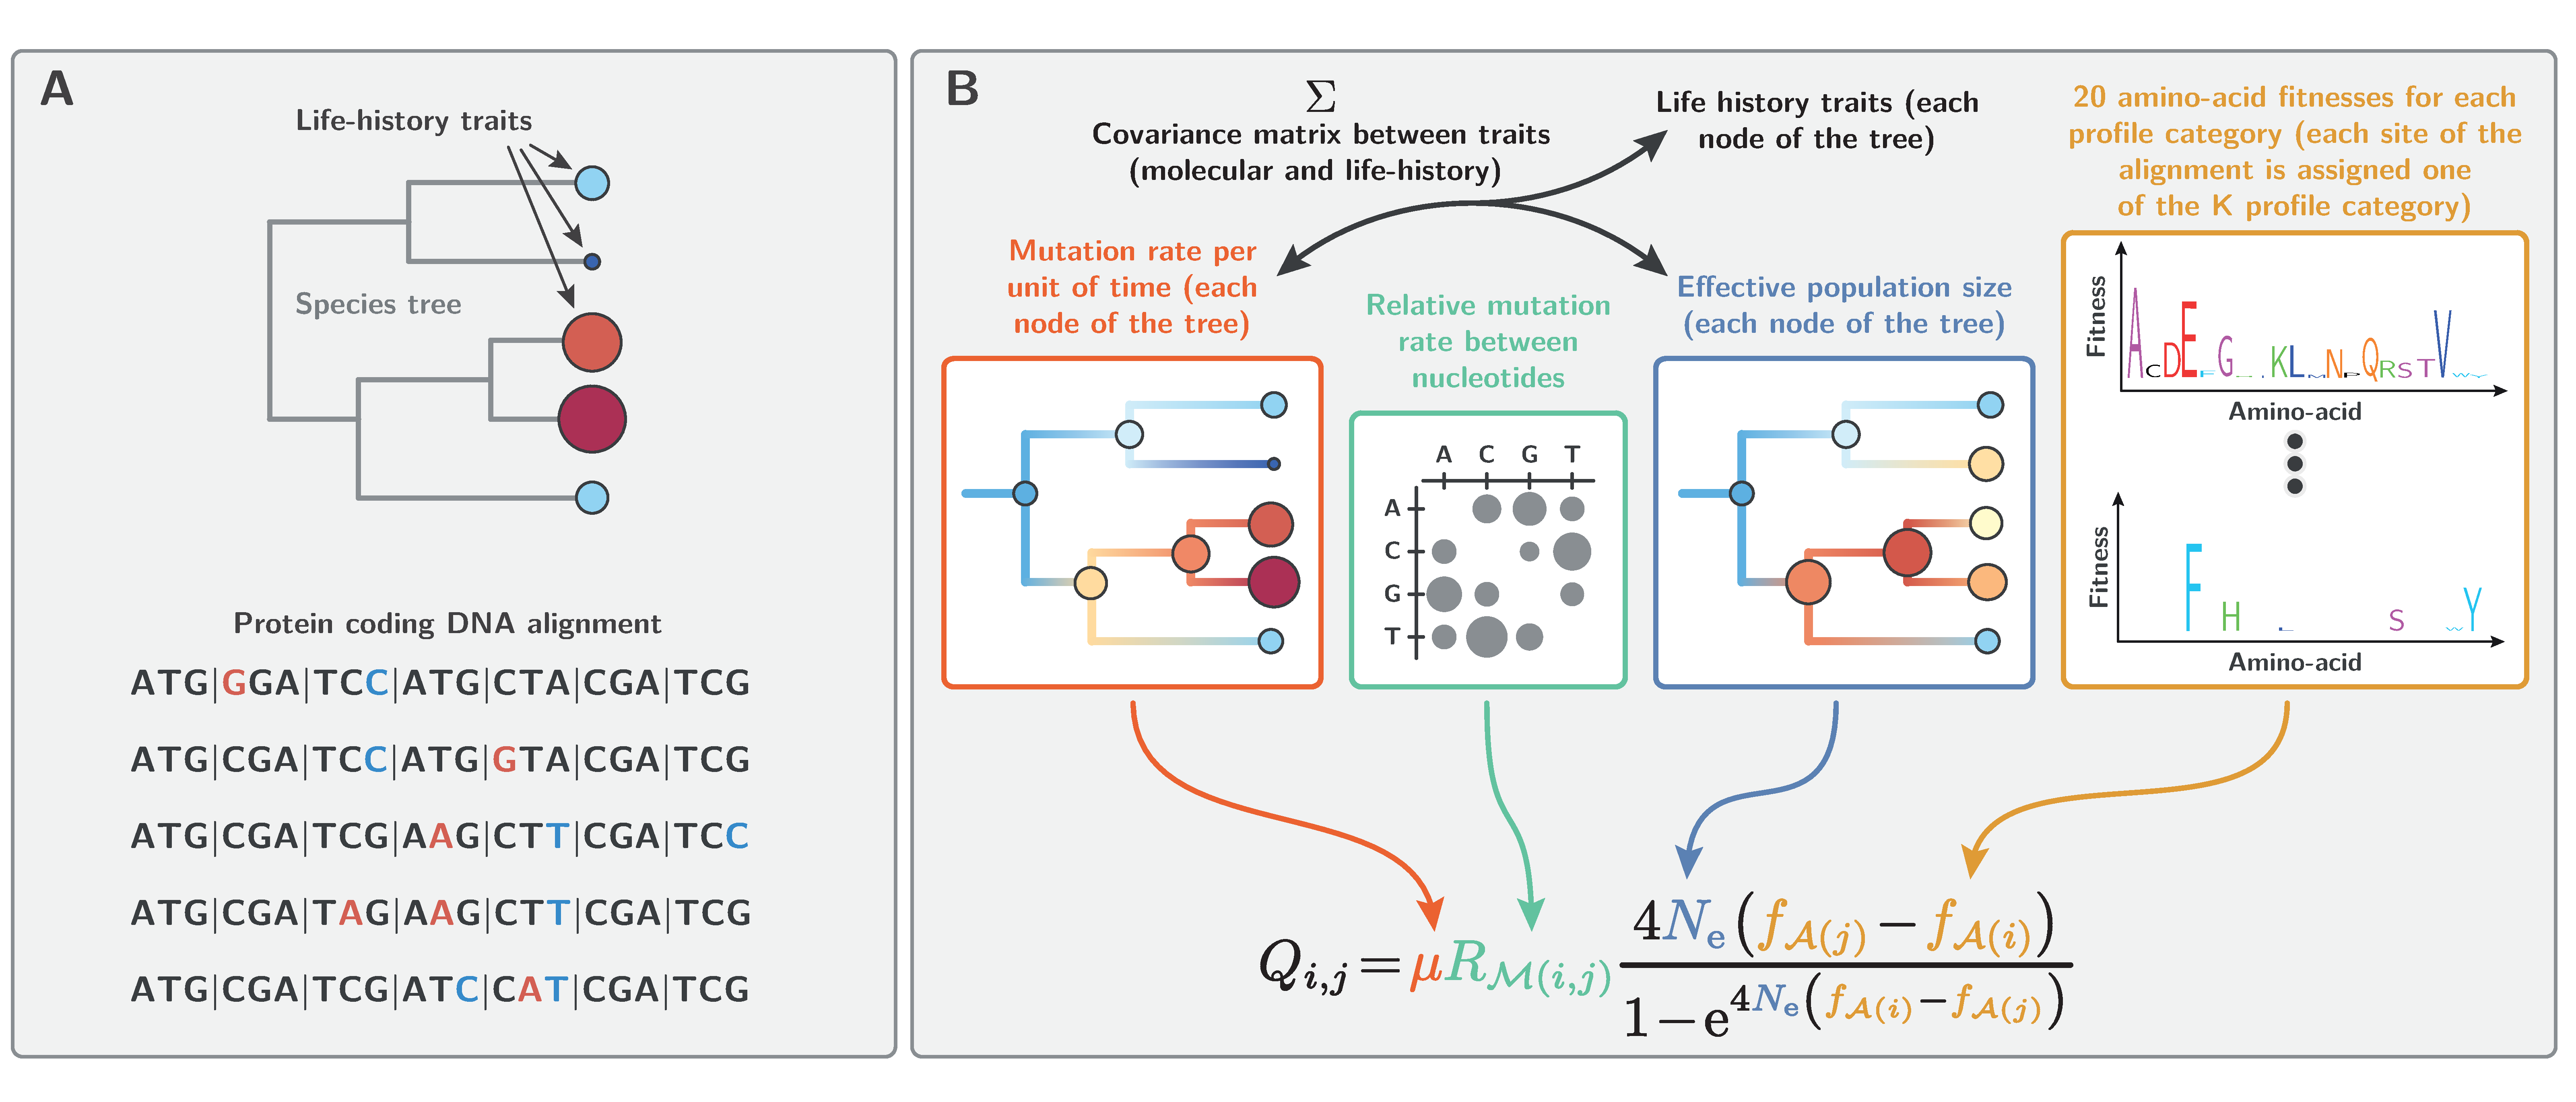
\includegraphics[width=\textwidth] {model_summary.pdf}
	\caption[Model summary]{
		Model summary.
		Panel A.
		Our method requires a given rooted topology, and an alignment of protein coding \acrshort{DNA} for the extant species.
		Optionally, the method can use quantitative life-history traits at the leaves of the tree, and dated estimation for the internal nodes of the tree.
		Panel B.
		Our Bayesian inference model estimates selection coefficients, mutation rate, intensity of random drift and the age of the internal nodes.
		Effective population since~($\Ne$) and mutation rate per unit of time~($\mu$) are considered fluctuating branch-wise, but assumed constant across all sites of the \acrshort{DNA} sequence.
		Conversely, the selection coefficient of amino-acids are considered changing for sites along the \acrshort{DNA} sequence, but are considered constant across the tree.
		Branch-heterogeneity is modeled as an auto-correlated log-Brownian process, meaning our model estimates correlation coefficients between quantitative traits (as input), $\Ne$, and $\mu$, where phylogenetic inertia is accounted for.
		Synonymous \glspl{substitution} are leveraged to estimates branch-wise mutation rate~($\mu$).
		Site-specific rates of \glspl{non-synonymous} across the tree is leveraged to estimate site-wise selection coefficient~($\Fit$).
		Branch-specific rates of \glspl{non-synonymous} across the sequence is leveraged to estimate branch-wise random drift~($\Ne$).
	}
	\label{fig:modelSummary}
\end{figure}

\subsection{Substitution rate equation}
\label{sec:MutSelEq}
DNA coding sequences are modeled at the level of the \gls{codon}, where for each site (counted by triplets in the alignment), a change of \gls{codon} means a change in \acrshort{DNA} but not necessarily in amino-acid.
The \gls{substitution} rate (per unit of time) from \gls{codon} $\ci$ to $\cj$, denoted $\submatrix_{\itoj}$, is equal to the total rate of mutation (per unit of time) at the level of the population~($2\Ne\mu_{\itoj}$) multiplied by the probability of fixation of the mutation:
\begin{equation}
{\submatrix_{\itoj}} = 2 \Ne \mu_{\itoj} p_{\mathrm{fix}}(\itoj)
\end{equation}

In the case of synonymous mutations, which we assumed are \gls{neutral}, the probability of fixation is independent of the original and target \gls{codon}, and equal $1/2 \Ne$.
Finally ${\submatrix_{\itoj}}$ simplifies to: 
\begin{equation}
\submatrix_{\itoj} = \mu_{\itoj}
\end{equation}

In the case of non-synonymous mutations, the probability of fixation depends on the difference in fitness between the amino-acid encoded by the initial and final \glspl{codon}~\citep{Ohta1992}:
\begin{equation}
\label{eq:mutationSelection}
{\submatrix_{\itoj}} = \mu_{\itoj} \dfrac{4 \Ne \left({\fitj - \fiti}\right)}{{1 - \e^{4 \Ne \left({\fiti - \fitj}\right)} }}
\end{equation}
where $\Fit$ is a $20$-dimensional vector specifying the log-fitness for each amino-acid, and $\aai$ is the amino-acid encoded by \gls{codon} $i$.
We see from this equation that, $\fit$ and $\Ne$ are confounded, such that increasing the \gls{effective-population-size} while decreasing the fitnesses by the same factor leads to the same \gls{substitution} rate.

The mutation rate $\mu_{\itoj}$ depends on the underlying nucleotide change between the \glspl{codon} $\ci$ and $\cj$.
First, if \gls{codon} $\ci$ to $\cj$ are not neighbors, $\mu_{\itoj}$ is equal to $0$.

Second, if \gls{codon} $\ci$ and $\cj$ are only one mutation away, $\mu_{\itoj}$ is given by the nucleotide relative rate~(${\mutmatrix_{\nucitoj}}$) scaled by the mutation rate per time~($\mu$).
Technically, the $4$-dimensional nucleotide relative rate matrix~($\Mutmatrix$) is normalized such that we expect $1$ \gls{substitution} per unit of time, hence the scaling by $\mu$.

\subsection{Site-selection model}
\label{sec:SiteHetero}
The strength of selection is not typically homogeneous along the sequence.
For example, exposed sites are under lower selective pressure than buried sites~\citep{Echave2016}.
In fact, selection differs in a way that depends on the local physico-chemical requirements~\citep{Goldstein2016,Goldstein2017,Weber2019}.
Following the seminal work on mutation-selection models~\citep{Halpern1998}, one increasingly popular way to account for this variation is to allow for site-specific amino-acid fitness profiles (20-dimensional vectors).

The sparcity of signal per site requires to aggregate sites together in categories, such as to fit the amino-acid fitnesses.
Conversely, the category assigned to each site is fitted such that the sites aggregated into the same category share the pattern of selection and hopefully the same physico-chemical properties.
The methods previously developed to estimate site-heterogeneous amino-acid fitnesses relied on penalized-likelihood~\citep{Tamuri2012,Tamuri2014}, or a Bayesian non-parametric random-effect approach~\citep{Rodrigue2010,Rodrigue2014,Rodrigue2016}.
The work presented here relies on the Bayesian approach, as in \textit{PhyloBayes}~\citep{Rodrigue2010}.

\subsection{Branch-traits model}
\label{sec:BranchHetero}
Many phenotypic traits can vary between species, either evolutionary parameters of interest, environmental variables or life-history traits~\citep{Felsenstein1985,Romiguier2014}.
However, the value of a trait along a branch is expected to be dependent on the value at the parent branch, such that abrupt shifts on trait value should be penalized~\citep{Huelsenbeck2003,Seo2004}.
Moreover, some of these traits might be correlated, for example an increase in $\Ne$ might be correlated with a decrease in body size~\citep{Weber2014,Romiguier2014}.

Correlation of traits has previously been modeled using diffusive log-Brownian multivariate process along a phylogeny~\citep{Seo2004,Lartillot2011}.
Under a log-Brownian process, the logarithm of the trait value at a given node of the tree is normally distributed, with mean equal to the log-value at parent node, and the standard deviation is proportional to the branch size (in unit of time).

In a multivariate process, traits are modeled together as a vector-valued time-dependent random process, parameterized by a covariance matrix between traits~($\Covariancematrix$).
Altogether, values of the multivariate process at each node of the tree, a covariance matrix and divergence times are jointly estimated.
Once the traits are sampled at all nodes, traits along each branch is taken as the average (see Methods) between extremities of this branch.
The work presented here implemented the branch-heterogeneity in a Bayesian context, as in \textit{CoEvol}~\citep{Lartillot2011}.
Technically, the precision matrix (invert of covariance matrix) is distributed as an invert Wishart, meaning the \gls{prior} matrix is diagonal pushing the correlation coefficients toward $0$.

\subsection{Mutation-selection-random drift model}
\label{sec:BranchSiteHetero}
Our Bayesian inference model (see Methods) can be viewed as an integration between mutation-selection models accounting for site-heterogeneity of selection coefficients, and the molecular comparative approach accounting for variation in molecular and phenotypic or life-history traits between species.
More specifically, in the model now presented, $\Ne$ and $\mu$ are allowed to vary between species (across branches), but assumed constant along the \acrshort{DNA} sequence.
Conversely, amino-acid fitness profiles are assumed to vary across sites, but are considered constant along the tree (Figure~\ref{fig:modelSummary}).

The phylogenetic \gls{codon} model presented here makes several additional assumptions on the evolutionary processes generating the observed alignment.
First, the species tree topology is supposed to be known, and each gene should match the species tree, meaning genes are strict orthologs (no paralogs and no horizontal transfers).
Second, there is no epistasis (interaction between sites), such that any position of the sequence has its own independent evolutionary process and a \gls{substitution} at one position does not affect the \gls{substitution} process at other positions.
Third, from a population genetic perspective, we assumed sites of the protein to be unlinked, or equivalently the mutation rate is low enough such that there is no Hill-Robertson interference nor genetic hitch-hiking.
Fourth, we assume \acrshort{DNA} sequences to be representative of the species, not taking into account the sampling effect tending to over-represent weakly deleterious mutations present at low frequencies.


Our Bayesian implementation, written in C++ is publicly available at \url{https://github.com/bayesiancook/bayescode/tree/chronogram}.

\begin{figure}[htb]
	\centering
	\begin{minipage}{0.32\linewidth}
		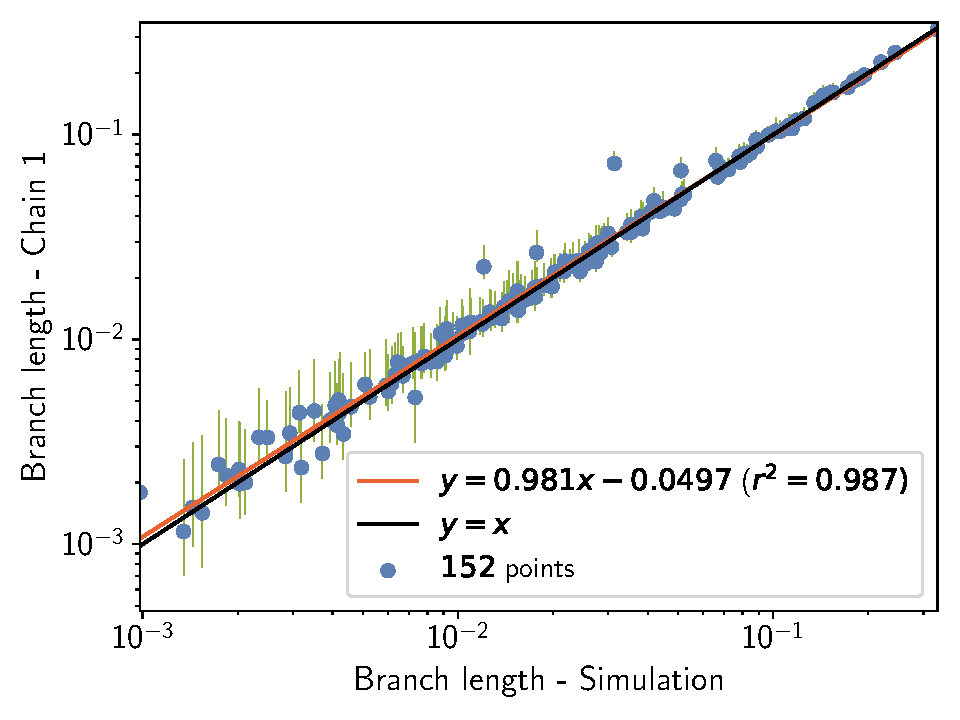
\includegraphics[width=\linewidth, page=1]{simulations/BranchWise_SimuDiv_SiteMutSelBranchNe_BranchCorrelation_Log10BranchLength}
	\end{minipage}	\hfill
	\begin{minipage}{0.32\linewidth}
		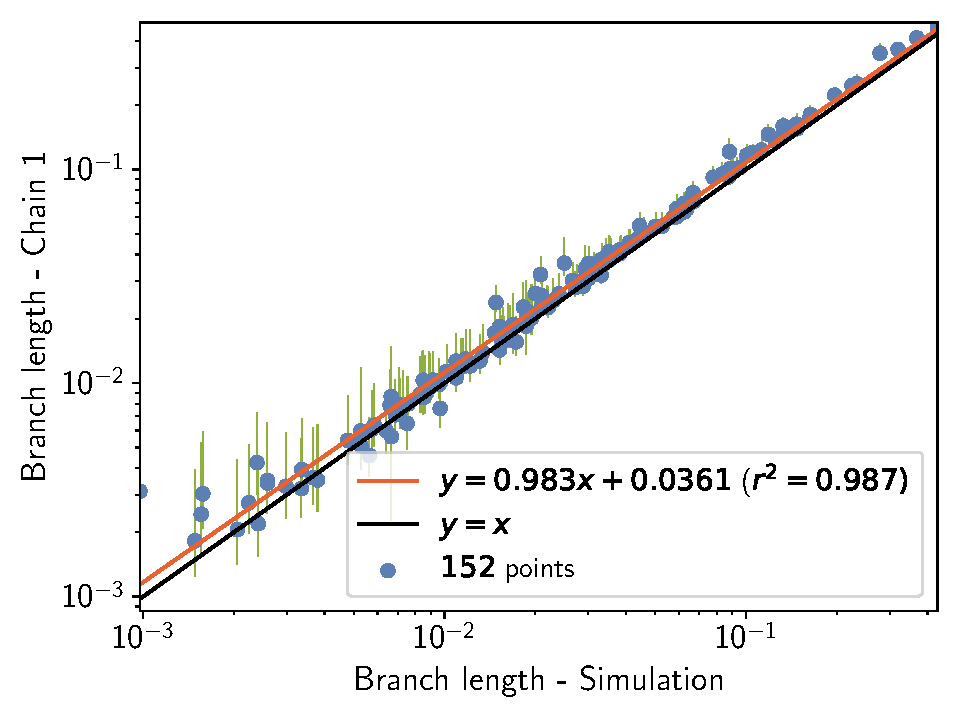
\includegraphics[width=\linewidth, page=1]{simulations/SimuPoly_SiteMutSelBranchNe_BranchCorrelation_Log10BranchLength}
	\end{minipage}	\hfill
	\begin{minipage}{0.32\linewidth}
		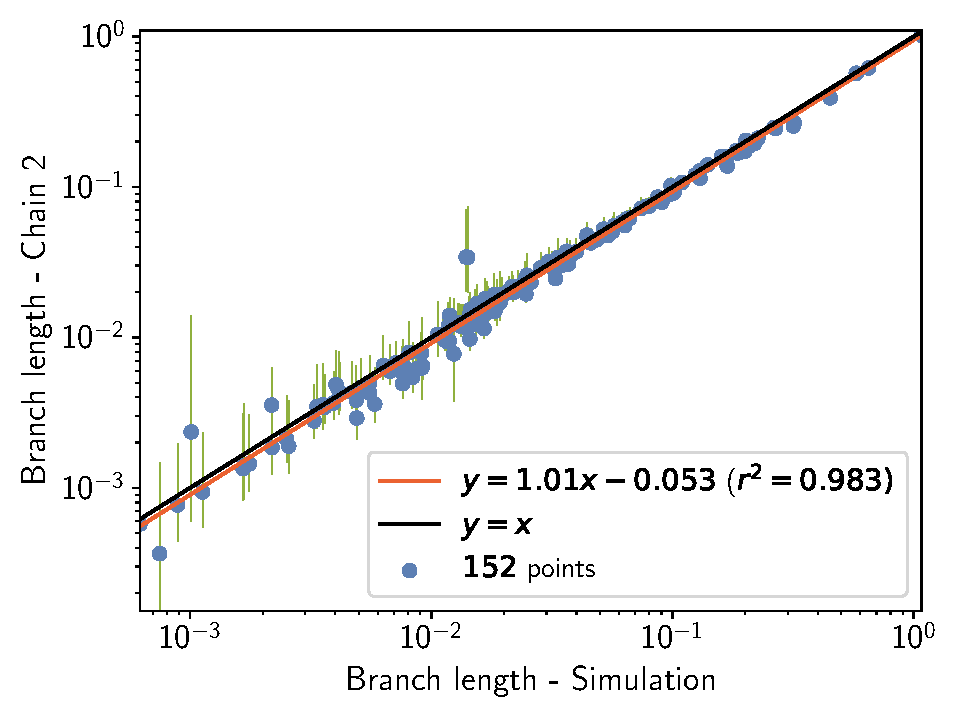
\includegraphics[width=\linewidth, page=1]{simulations/SimuGeo_SiteMutSelBranchNe_BranchCorrelation_Log10BranchLength}
	\end{minipage}	\hfill
	\begin{minipage}{0.32\linewidth}
		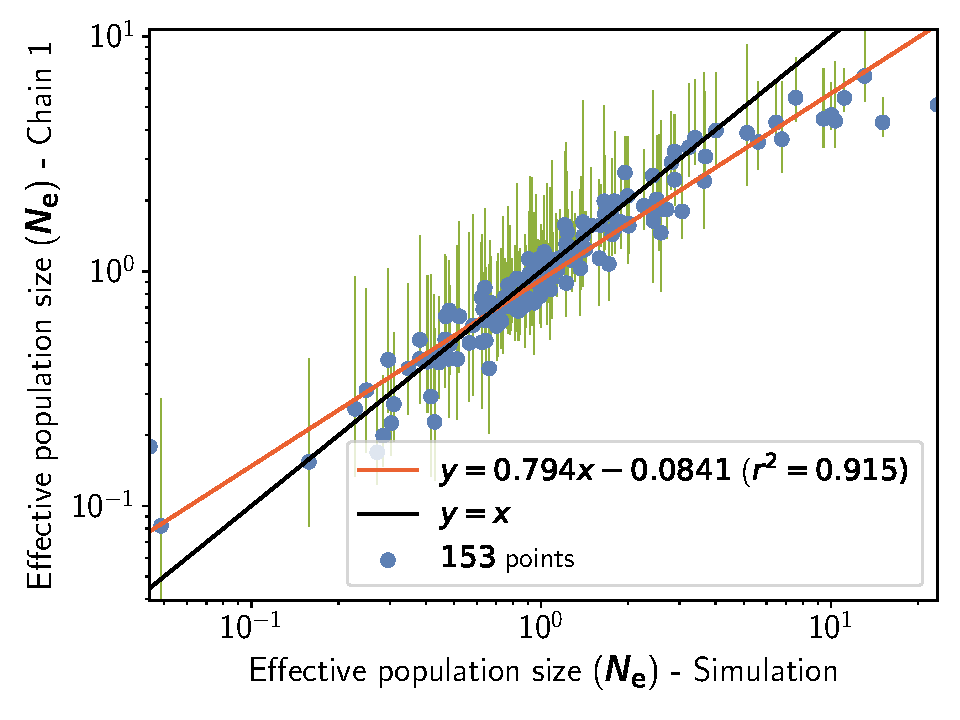
\includegraphics[width=\linewidth, page=1]{simulations/BranchWise_SimuDiv_SiteMutSelBranchNe_BranchCorrelation_LogPopulationSize}
	\end{minipage}	\hfill
	\begin{minipage}{0.32\linewidth}
		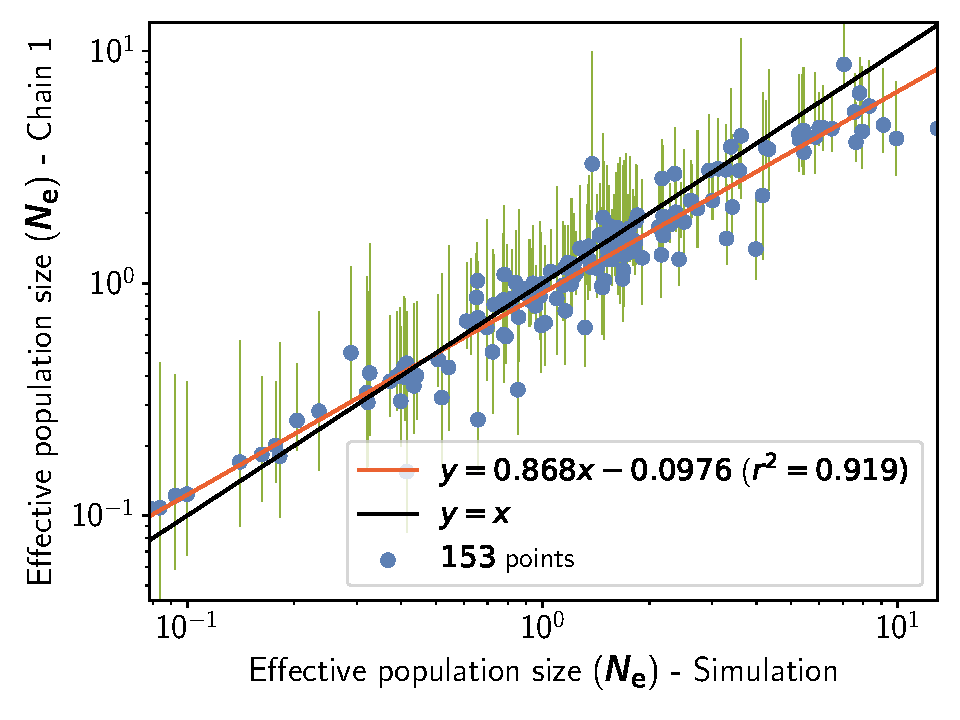
\includegraphics[width=\linewidth, page=1]{simulations/SimuPoly_SiteMutSelBranchNe_BranchCorrelation_LogPopulationSize}
	\end{minipage}	\hfill
	\begin{minipage}{0.32\linewidth}
		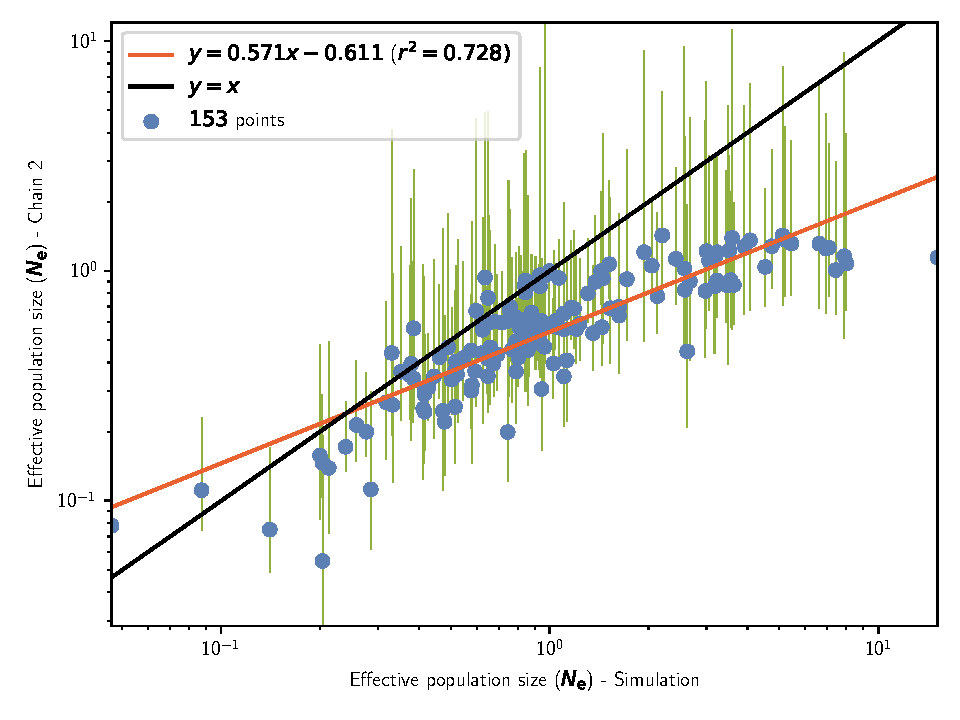
\includegraphics[width=\linewidth, page=1]{simulations/SimuGeo_SiteMutSelBranchNe_BranchCorrelation_LogPopulationSize}
	\end{minipage}	\hfill
	\caption[Inferred and simulated $\Ne$]{
		Inferred and simulated $\Ne$
		Top row, branch length in expected number of \glspl{substitution}, for each branch of the tree.
		Bottom row, $\Ne$ for each node (including leaves) of the tree, relative to $\Ne$ at the root of the tree.
		Left panel, simulation under the mutation-selection approximation, as to test the soundness of the inference framework.
		Middle panel, simulation accounting for small population size effects~($5000$ individuals at the root), site linkage and short term fluctuation of $\Ne$.
		Right panel, simulation accounting for site epistasis, with fluctuation of the selection coefficient along the phylogeny.
		The tree root is $150$ million years old, where the initial population start with a mutation rate of $\smash{1e^{-8}}$ per site per generation, and generation time of $10$ years.
		These experiments confirm that signal in the placental mammalian tree can allow to reliably infer the direction of change in $\Ne$, even if linkage disequilibrium, short term fluctuation of $\Ne$ and finite population size effects are not accounted for in the inference framework.
		However, the presence of epistasis between sites is a serious threat to the inference of $\Ne$.
	}
	\label{fig:simulations}
\end{figure}

\section{Results}
\label{sec:Results}

\subsection{Simulated experiments}
\label{sec:ResultsSimulated}
The inference framework was first tested using independently simulated alignments (see Methods).
With the aim of applying the inference method to empirical dataset in placental mammals and in primates, the simulation parameters were chosen to match the empirical regime of total branch length (expected number of substitutions) from root to leaves.

A first serie of simulations was meant to test the soundness of our inference framework, by simulating essentially under the model used for inference.
The mutation-selection approximation was assumed to be valid, and sites were simulated under different fitness profiles.
In addition, $\Ne$ varies at the tree nodes but otherwise remains constant along each branch.
In this context, simulated branch length and $\Ne$ could be recovered appropriately by our inference method (Figure~\ref{fig:simulations}, panel A \& B).
Unfortunately, assumptions made for this simulations are almost certainly violated in practice.
First, $\Ne$ should change continuously along a branch, between each generation of the population.
Second, having a separate process for each site is equivalent to have no linkage between sites (free recombination), an assumption that should be relaxed. 
Third, the probability of fixation (equation \ref{eq:mutationSelection}) does not hold in small finite population.

For these reasons, we performed a second more challenging series of simulations.
The finite population was modeled explicitly in a Wright-Fisher simulator, tracking the frequency of each \gls{allele} at each generation along the phylogeny.
Such simulator accounts for small population size effects, hitchhiking of weakly deleterious mutations during selective sweep and background selection due to linkage desequilibrium.
Fluctuations of $\Ne$ and mutation rate were also fluctuating continuously along the branch of the tree.
Moreover, noise was added by accounting for short term fluctuations of $\Ne$ on the order of $20\%$ per generation.
The simulated branch length and $\Ne$ could be robustly recovered by the inference framework in this context (Figure~\ref{fig:simulations}, panel C \& D).

However, if the results are encouraging to apply the method on empirical data, we rely on the assumption of site-independent fitness landscape, which is almost certainly broken in practice.
Finally, we implemented a more complex, site-dependent fitness landscape accounting for the $3$-dimensional structure of protein and interaction between sites.
In such a model, the folding energy of the protein determines the probability of being in the folded state, a proxy for fitness~\citep{Goldstein2017}.
During a simulation, at a particular \gls{codon} site, the fitness landscape is dependent on the actual amino-acids present in the vicinity of this particular site.
Our inference framework could recover the simulated branch length, but had more difficulties to retrieve the simulated $\Ne$ in the context of site-dependent epistasis (Figure~\ref{fig:simulations}, panel E \& F)

\subsection{Empirical experiments}
\label{sec:ResultsEmpirical}
\begin{figure}[H]
	\centering
	\begin{minipage}{0.411\linewidth}
		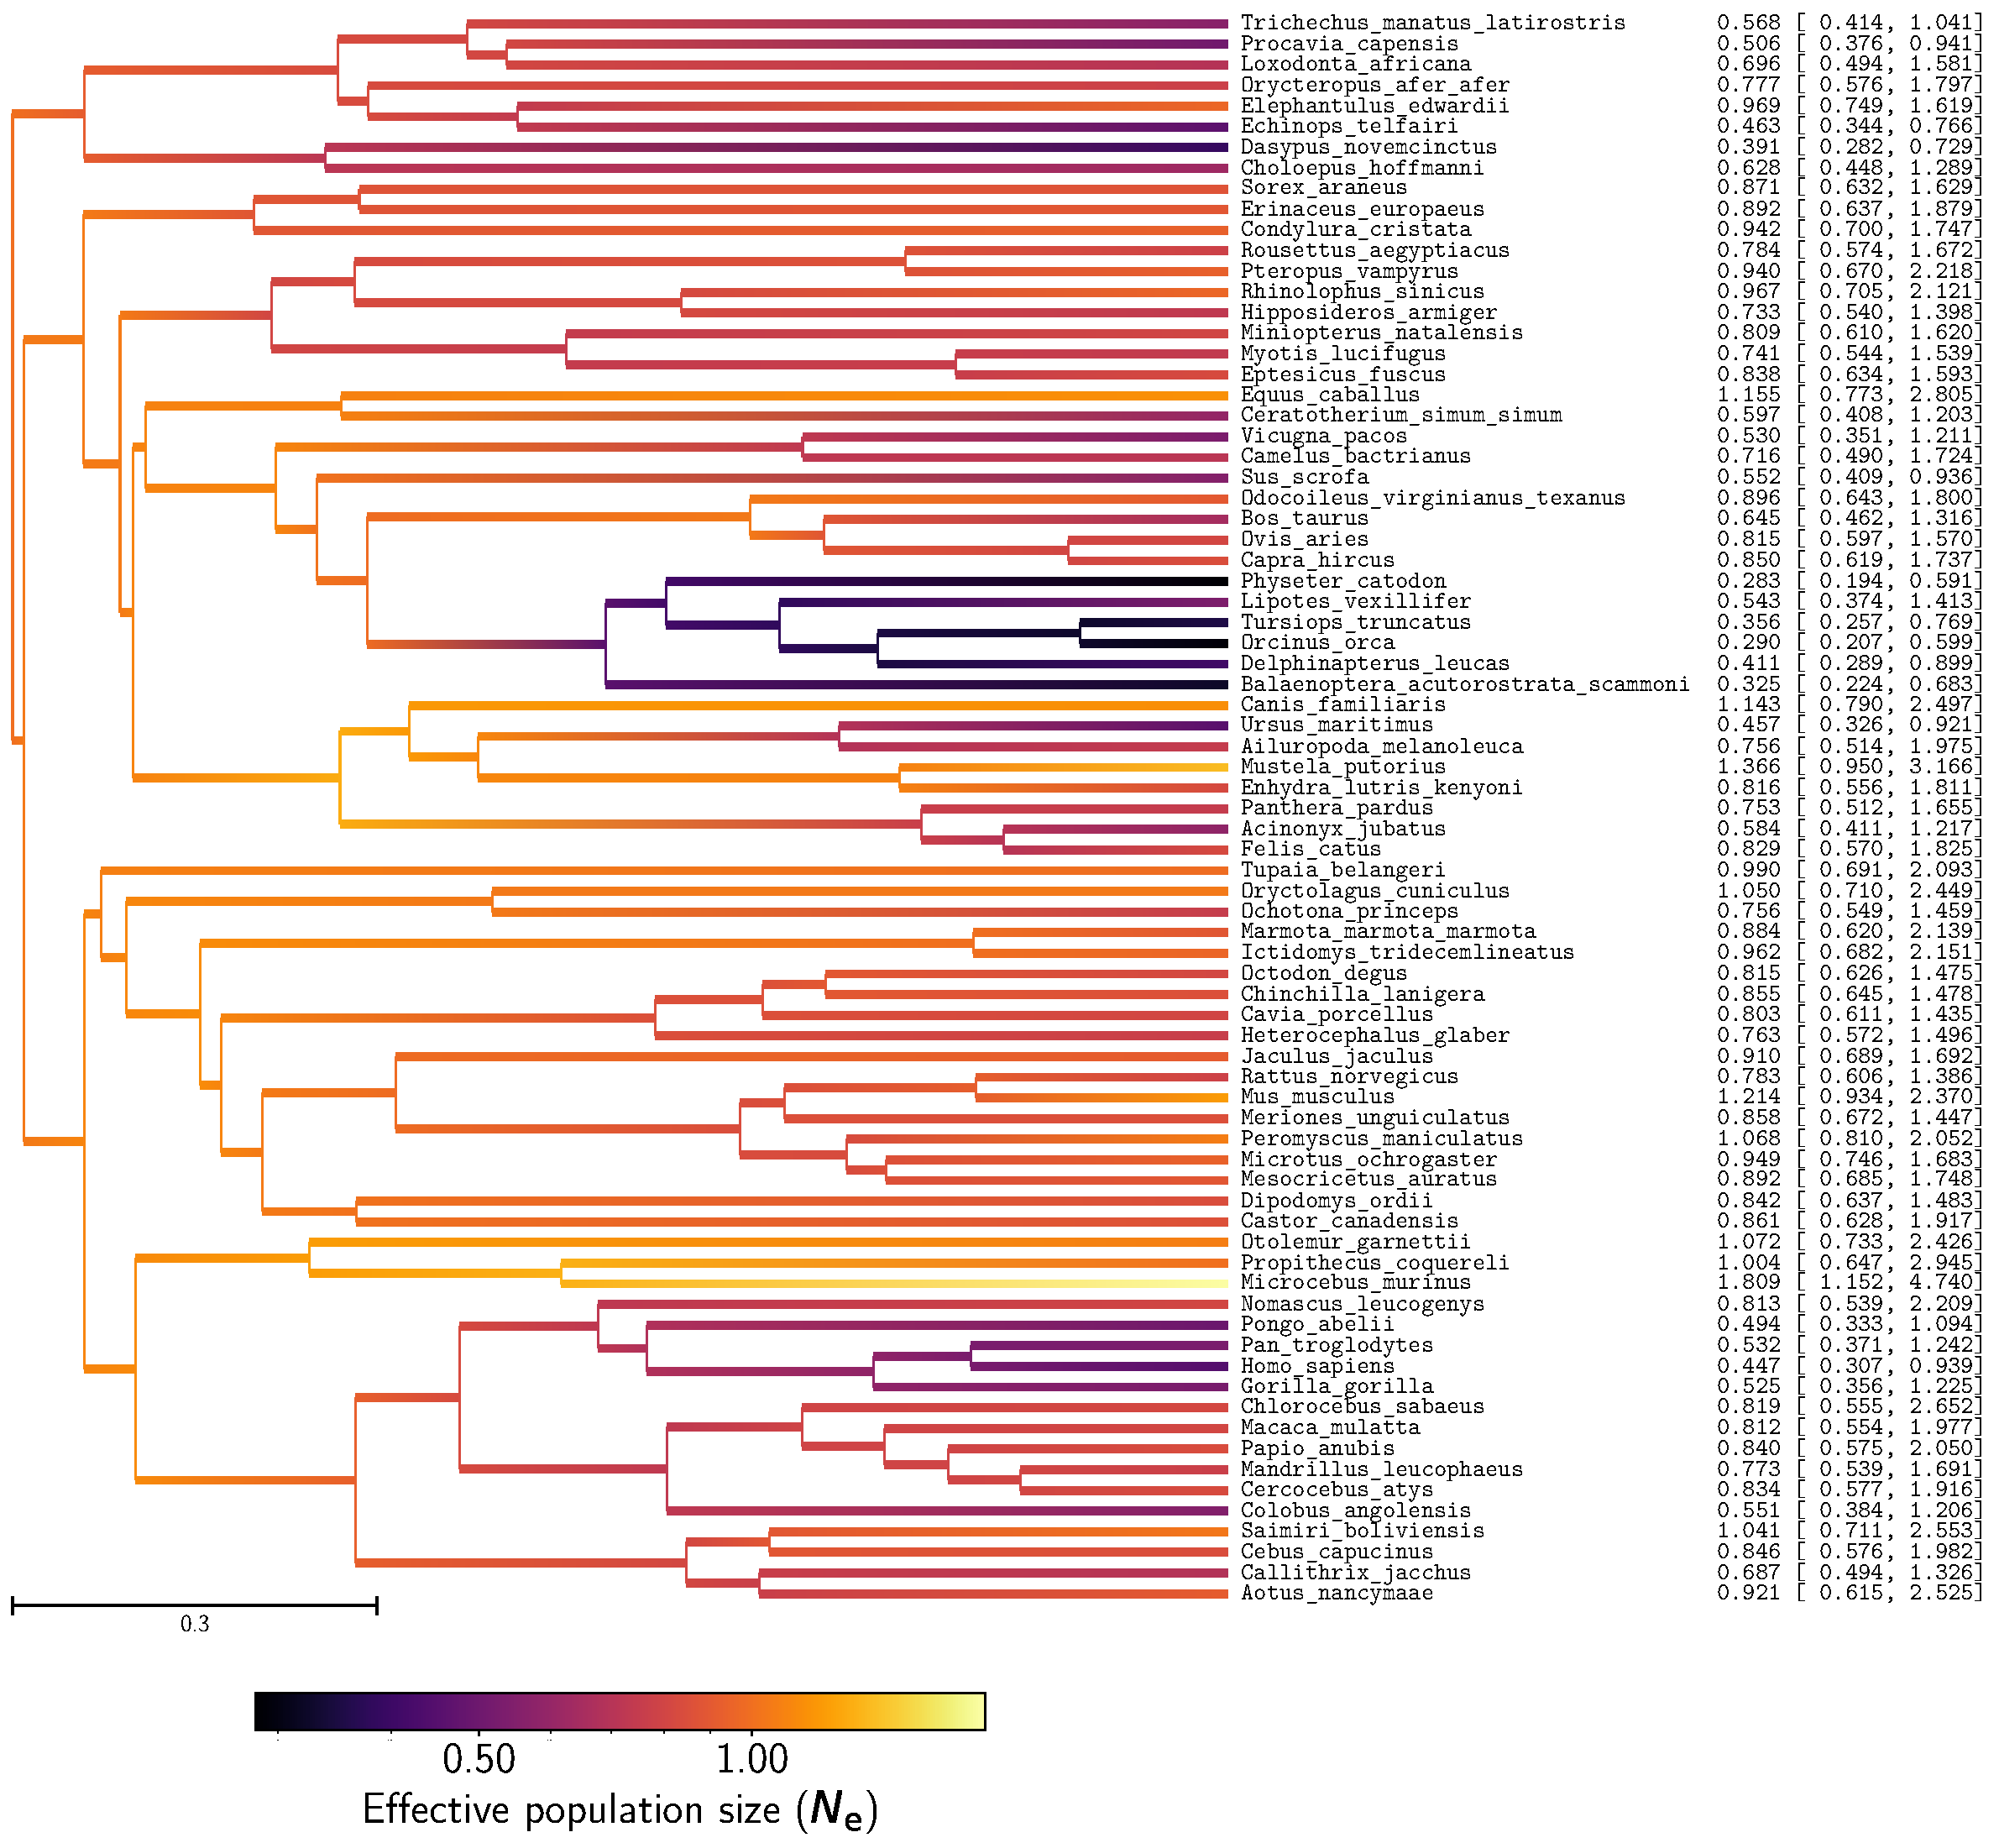
\includegraphics[valign=t, width=\linewidth, page=1, clip, trim=0cm 0cm 15.35cm 0.15cm]{mammals/18CDS_SiteMutSelBranchNe_R1_LogPopulationSize}
	\end{minipage}
	\begin{minipage}{0.158\linewidth}
		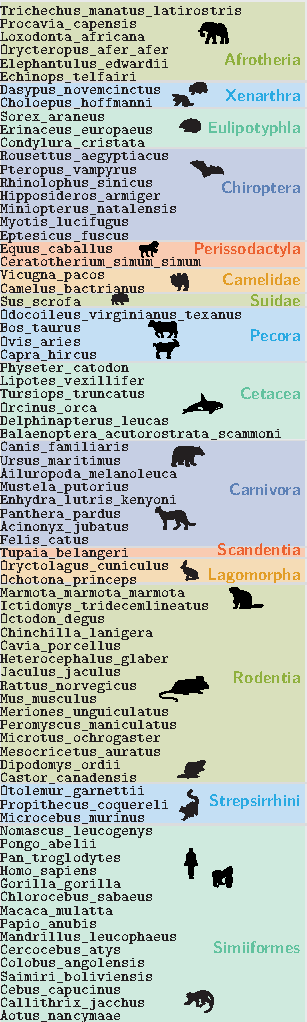
\includegraphics[valign=t, width=\linewidth, page=1, clip, trim=0cm -2.2cm 0cm 0cm]{mammals_species}
	\end{minipage}
	\begin{minipage}{0.411\linewidth}
		\reflectbox{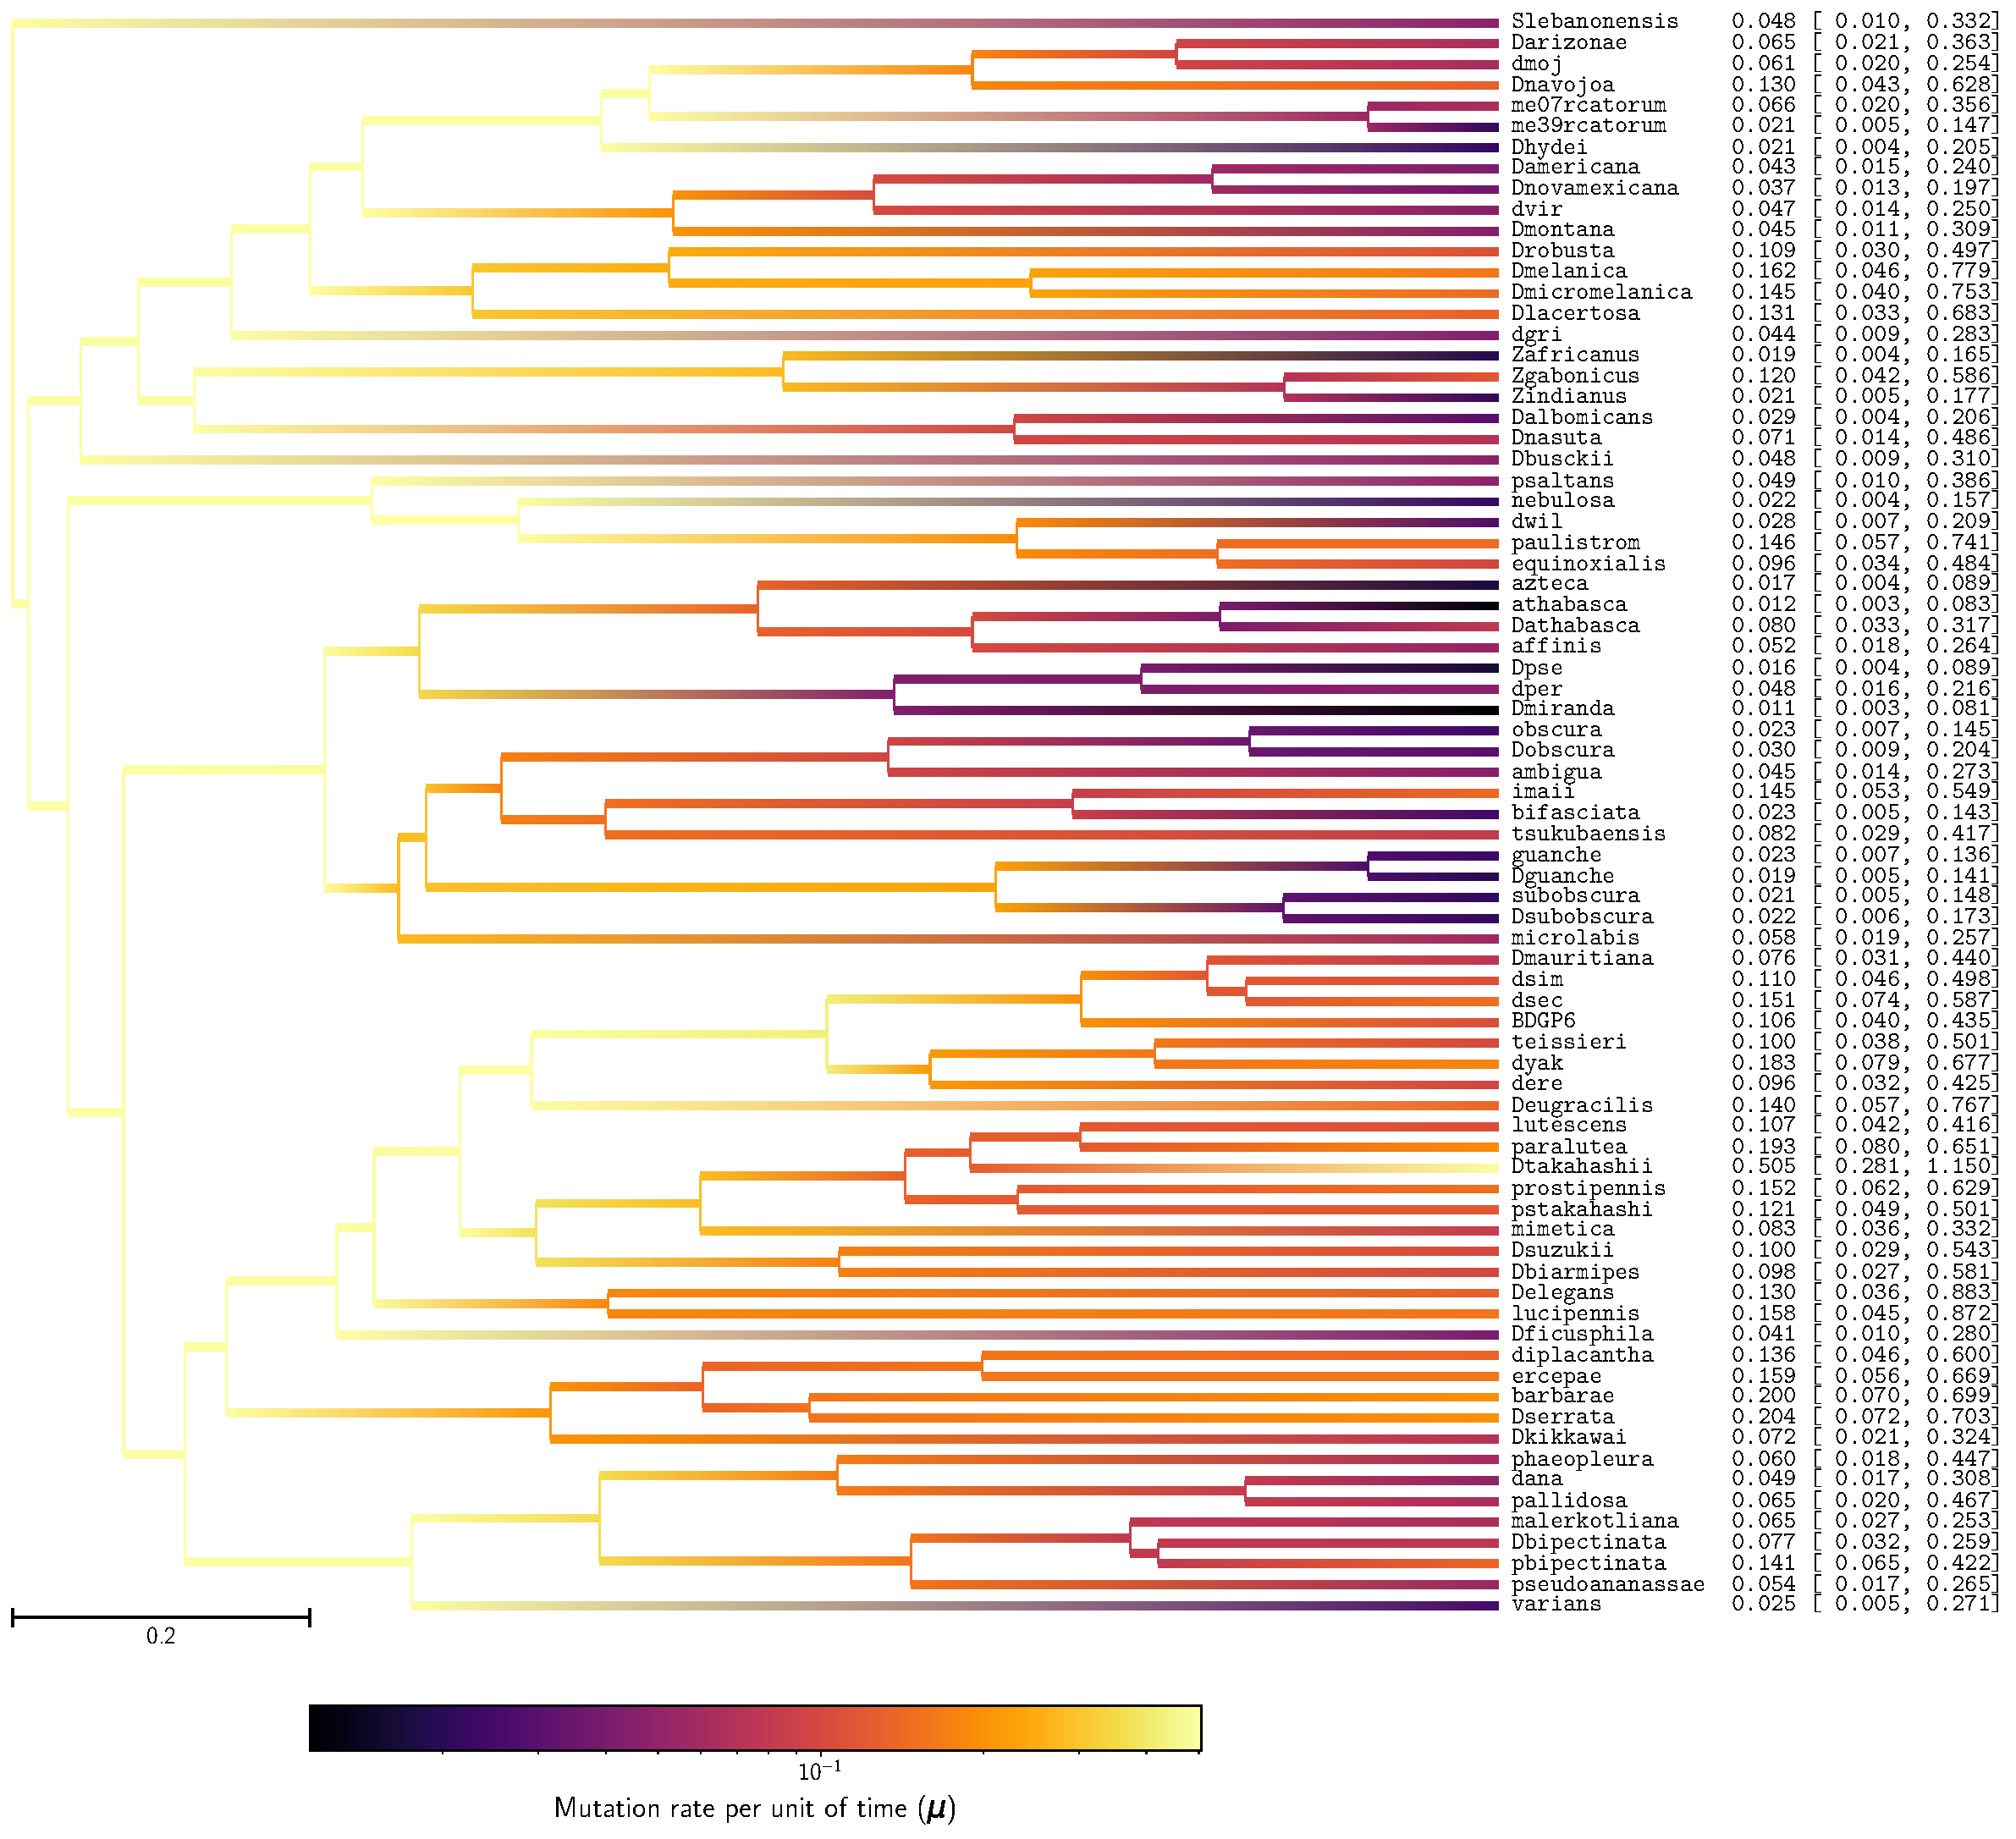
\includegraphics[valign=t, width=\linewidth, page=1, clip, trim=0cm 4.48cm 15.35cm 0cm]{mammals/18CDS_SiteMutSelBranchNe_R1_LogMutationRatePerTime}}
		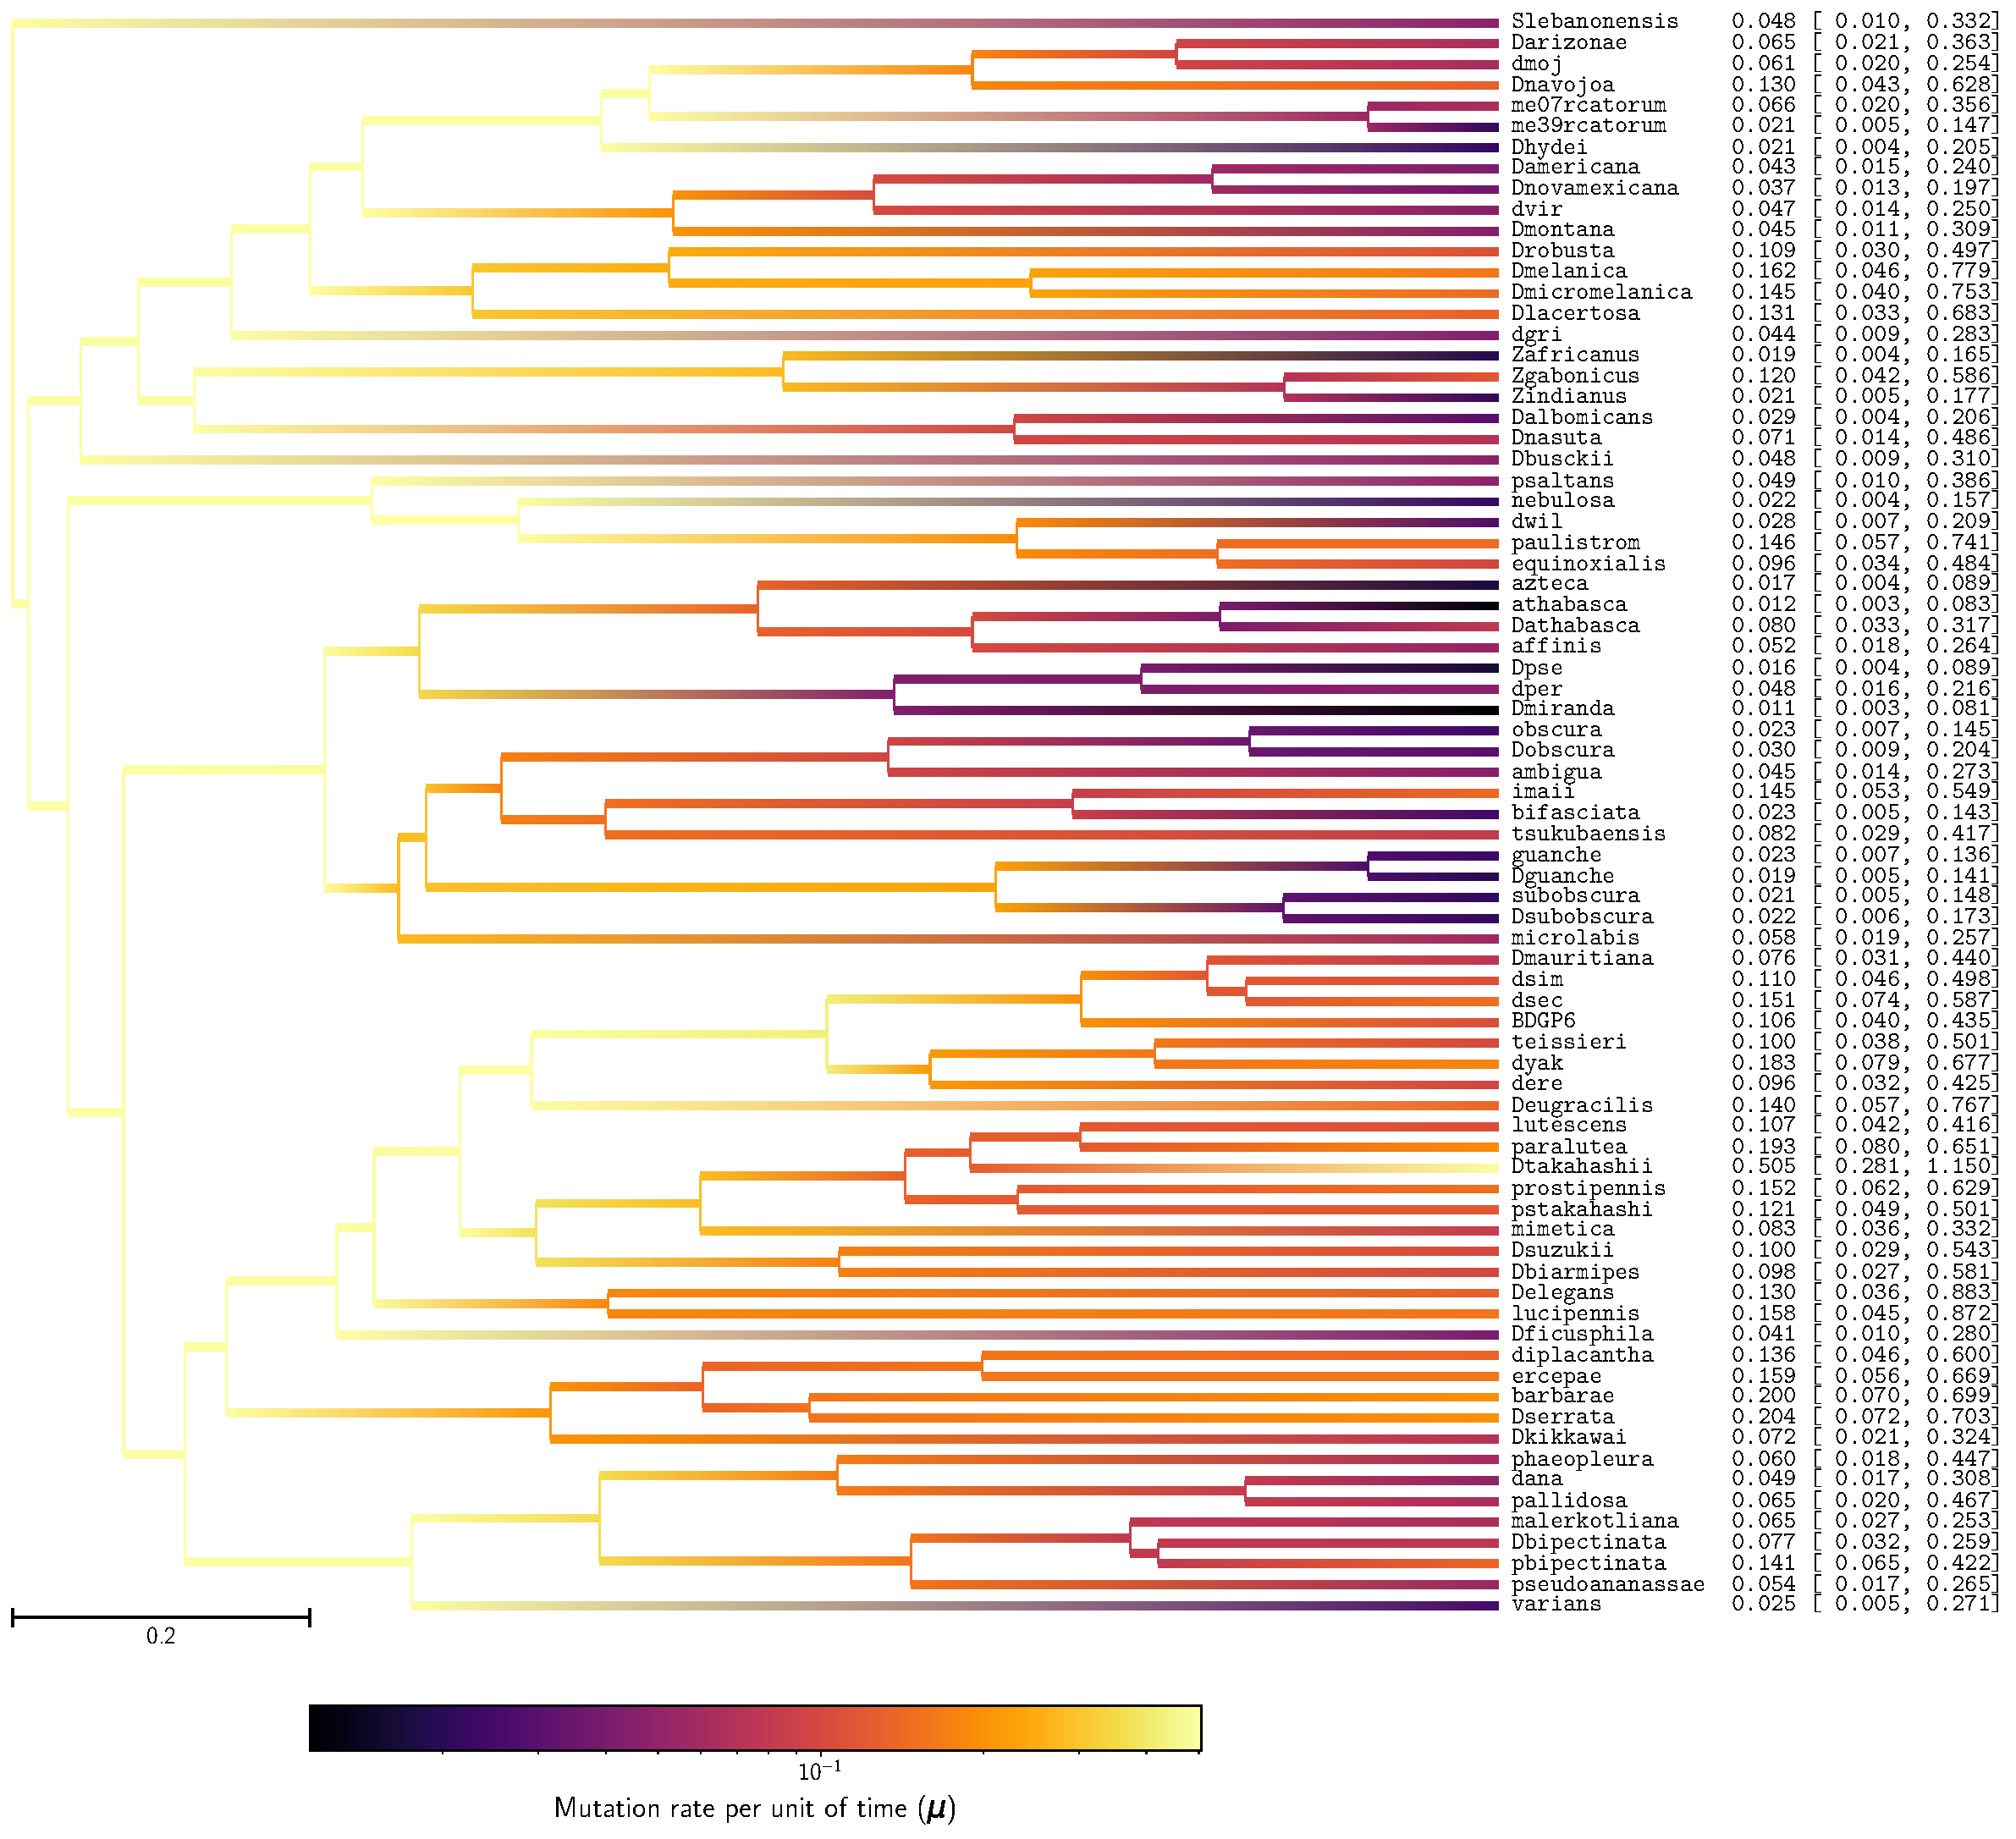
\includegraphics[valign=b,width=\linewidth, page=1, clip, trim=0cm 0cm 15.35cm 32.3cm]{mammals/18CDS_SiteMutSelBranchNe_R1_LogMutationRatePerTime}
	\end{minipage}
	\caption[Example of inferred $\Ne$ and $\mu$ on placental mammals dataset]{
		Example of inferred $\Ne$ and $\mu$ on placental mammals dataset.
		Inference were performed on a randomly chosen set of $36$ coding sequences (CDS) out of $226$ highly conserved CDS~($<1\%$ of gaps).
		Only highly conserved CDS were retained such that the assumption of constant fitness landscape is not incautiously broken by protein with changing function and/or adaptive selection.
		Brownian processes along the tree are represented for effective population size~($\Ne$, left panel) and mutation rate per site per unit of time~($\mu$, right panel).
		Mean values of \acrshort{MCMC} (after burn-in) are obtained at each node of the tree, hence a gradient can be extrapolated along each branch.
		At each node, the inner circle represent the lower bound of the \acrshort{MCMC} $90\%$ confidence interval, and the outer circle represent the upper bound, as to give visual input into the range of estimation.
		$\mu$ spanned almost $2$ order of magnitude, and if we assume the root to be $105$My old~\citep{Kumar2017}, the re-scaled mutation rate per site per year in extant species is between $\smash{1.1e^{-10}}$ and $\smash{7.8e^{-9}}$.
		$\Ne$ at the root of the tree is arbitrarily set to $1$, and all values are relative to the root.
	}
	\label{fig:mammals_popsize_and_mutrate}
\end{figure}

We reconstructed long-term changes of effective population size~($\Ne$) and mutation rate per site per unit of time~($\mu$) in placental mammals, with alignments extracted from OrthoMam database~\citep{Ranwez2007,Scornavacca2019}.
Life-history traits (LHT) for longevity, age at maturity and weight were obtained from AnAge database~\citep{DEMAGALHAES2009,Tacutu2012}.
We focused our analysis on 77 taxa for which information is available for at least one LHT.

In the result of this analysis (Figure~\ref{fig:mammals_popsize_and_mutrate}), we visually observe a global trend of increased $\Ne$ throughout the tree around $90$ and $60$ My.
We also observe $\Ne$ to be lower in \textit{Cetacea} and \textit{Camelidae}, while being higher in \textit{Rodentia} and \textit{Pecora}.
In some clades we can see a decrease along a single branch of the tree, for example \textit{Heterocephalus glaber} or \textit{Acinonyx jubatus}.

The analysis of the covariance matrix, discarding phylogenetic inertia, shows that $\Ne$ is positively correlated~($r^2 = 0.44$) with mutation rate per unit of time (Table~\ref{fig:mammals_correlation}), which is compatible with the assumption that large population are small-sized and with a shorter generation time.
Moreover the \gls{effective-population-size} is negatively correlated with longevity, age at maturity and weight (Table~\ref{fig:mammals_correlation}), consistent with the observation that larger population have small-sized and short-lived individuals~\citep{Galtier2016,Romiguier2014}.
The partial-correlation coefficients (Supplementary Materials) are not significantly different from $0$.

However, if the trend of $\Ne$ would be in the right direction, the magnitude of inferred $\Ne$ is vastly underestimated by our method, with a ratio of $2.5$ between the maximum and minimum $\Ne$ in extant species (Figure~\ref{fig:mammals_popsize_and_mutrate}).

To assess the reproducibility of our inference, we analyzed a concatenated random sample of 36 highly conserved coding sequences~($\leq 1\%$ of gaps in the alignment), and repeated the procedure on different random samples of 36 CDS.
Overall the estimation of $\Ne$ is reproducible for a random subset of CDS (Figure~\ref{fig:mammals_repeatability}).

\begin{table}[H]
	\centering
\noindent\adjustbox{max width=\textwidth}{%
\begin{tabu}{|c||c|c|c|}
\hline
\textbf{Correlation ($\bm{\rho}$)} & $\bm{N_{\mathrm{e}}}$ & $\bm{\mu}$ & \textbf{LogGenomeSize}\\
\hhline{|=#=|=|=|}
$\bm{N_{\mathrm{e}}}$ & - & $-0.0623$ & $-0.144$\\\hline
$\bm{\mu}$ & - & - & $0.224$\\\hline
\textbf{LogGenomeSize} & - & - & -\\\hline
\end{tabu}}

	\caption[Traits correlation]{
		Correlation coefficient between effective population size~($\Ne$), mutation rate per site per unit of time~($\mu$), and life-history traits (Maximum longevity, adult weight and female maturity), taking account phylogenetic inertia.
		Correlation coefficient are between $-1$ and $1$.
		Asterisks indicate strength of support~($\smash{^{*}} pp > 0.95$, $\smash{^{**}} pp > 0.975$).
		Observed correlation are compatible with the interpretation that large populations are composed of small, short-lived individuals.
		Moreover if the mutation rate per generation is considered constant in first approximation, the mutation rater per unit of time is positively correlated to generation rate, hence to population size.
	}
	\label{fig:mammals_correlation}
\end{table}

\section{Discussion}
\label{sec:Discussion}
% Summary 
Mechanistic phylogenetic \gls{codon} models explicitly define the \gls{substitution} rates as function of the mutation rate, selection and random drift.
Applied on an alignment of \acrshort{DNA} coding sequence, the mechanistic model can estimate amino-acid fitness landscapes along the \acrshort{DNA} sequence.
On the other hand, molecular comparative framework reconstruct the joint evolution of life-history, molecular and population-genetics traits along the phylogeny, intrinsically including phylogenetic inertia.
Combined together, the resulting framework can reconstruct site-heterogeneous amino-acid fitness landscapes, also the age of internal nodes, and finally reconstruct branch-heterogeneous life-history traits, $\mu$ and $\Ne$, with their correlation.
Testing the method against simulated alignments suggests the signal is strong enough in protein coding \acrshort{DNA} alignment to infer selection at the site level, and long-term changes in $\Ne$ and $\mu$ using a phylogenetic approach.
In placental mammals, $\Ne$ correlates negatively with longevity, weight and maturity, and positively with $\mu$.
Our observations suggest that the empirical signal is strong enough such that we can infer the directional trends in changes.

% Longvariance in Ne 
If the trend is in right direction, the magnitude of the change is greatly inferior to independent estimates.
Different mechanism not accounted for by the model could explain such a low variance of $\Ne$ inferred.
First, genetic hitch-hiking, Hill-Robertson interference, and short-term fluctuations of $\Ne$ could generate this effect.
However, inference on simulations tends to show their effect is not strong enough in the regimes explored.
Second, $\mu$ and $\Ne$ could also be fluctuating along the genome.
This assumption needs to be tested, though we expect that relaxing this assumption would not change drastically the magnitude of inferred $\Ne$.
Third, the \acrshort{DNA} sequences could also be misaligned in some sites, an effect we can control since the inferred $\Ne$ are repeatable for different set of genes.
Fourth, the genes selected in our alignments could be under adaptive evolution, or their function could have changed.
More precisely, the fitness profile at each site could change with time, either due to Red-Queen dynamics or due to epistasis because amino-acid \glspl{substitution} occurred at other sites.
Simulation of \acrshort{DNA} coding sequences under an epistatic landscape seemingly points to epistasis being the principal factor to be investigated, since $\Ne$ could not be appropriately inferred in such a case.
Independently, the magnitude of inferred $\Ne$ is quite similar for the placental mammals dataset and the primates dataset, while we would expect a greater discrepancy at longer phylogenetic scale.
An explanation could be that epistasis is more prevalent at longer time-scale, because the total number of \glspl{substitution} from root to leaves is greater, hence the fitness landscape is less stable.
Thought modeling epistasis in an inference framework is a complex biological, mathematical and computational problem, this work points to a potential signal of epistasis that could be retrieved in phylogenetic context.
% None equilibrium properties 

% Perspective : \gls{codon} bias
Our model also assume no bias in \gls{codon} usage, though the strength of selection for a particular \gls{codon} (or set of codons) among all synonymous possible \glspl{codon} has been proved to be substantial~\citep{Plotkin2011}.

This assumption can be relaxed by implementing \gls{codon} preferences that are shared across all sites, such that $41$ more parameters would be required in total.
Such implementation would provide the advantage of estimating \gls{codon} usage biases, and of accounting for its confounding effect while estimating selection and $\Ne$.

% Perspective: 
Bayesian computation shown in this study are based on relatively small alignments~($20,000$ sites at most), and with a limited parametrization in the number of fitness profile categories~($50$).
Analyzing execution duration of the program (not shown) leads to conclude that the number of fitness profile categories is the limiting step to expand the computation.
To estimate a more statistically stable genome-wide $\Ne$, we could develop an extended version leveraging parallel computing, where each coding sequence has its own computing process and own profile categories, but the $\Ne$ would be shared by all computing processes.
By increasing the number of categories per gene, the magnitude of inferred $\Ne$ would also increase, since fitness profiles would be sharper.

% Perspective: increase power
Mutation-selection models originated with the aim of increasing the power to detect adaptive evolution, by modeling explicitly the confounding effect of purifying selection.
However, by assuming constant $\Ne$ along a phylogeny, the statistical power to detect sites under adaptive evolution is not optimal.
Fitness profiles estimated are averaged along the phylogeny and are more seemingly \gls{neutral} than our estimated profiles under our present framework (Supplementary Materials).
Even though our method requires more computing resources to estimate fitness profiles, it provides a better null model of purifying selection to test against the presence of adaptive evolution.

% Comparison with other methods
Other methods have recently been developed to reconstruct phylogenetic changes in $\Ne$.
For example, a new method (preprint) uses \acrshort{DNA} coding sequences, a distribution of fitness effects, polymorphism and generation-time for some present-day species to reconstruct $\Ne$ along the phylogeny~\citep{Brevet2019}.
This method also based on the quasi-neutral theory of evolution allows to estimate the absolute value of $\Ne$, even for species where the polymorphism is unavailable.
Here our method requires neither generation time nor polymorphism, and the fitness effects are not constrained to a specific distribution.
However, the inferred values are solely relative and the computation requires more computing resources.
% Perspective: Short and long-term Ne

Estimating $\Ne$ in a mutation-selection phylogenetic model relies on the relation between $\Ne$ and relative strength of drift, where ultimately the signal of drift comes from the relative rate of \glspl{substitution}.
However, they do not leverage a second aspect of $\Ne$ at the population level, which determines the \gls{neutral} genetic diversity that can be maintained~($\pi=4\Ne \mu \tau$, where $\tau$ is the generation time).
Hence, \gls{polymorphic} data give us independent empirical estimates of $\Ne$, based on the assumption that mutations are \gls{neutral}.
In principle, our mechanistic model could be extended to leverage polymorphism within species in the case of differential selection, a method which has been previously pioneered in the case of $3$ species and using a distribution of fitness effect~\citep{Wilson2011}.
More generally, the \gls{nearly-neutral} theory of evolution defines a long-term $\Ne$, which might be different from the short-term definition of $\Ne$~\citep{Platt2018}.
Thus we could ask if empirical independent estimations of $\Ne$ from within species (polymorphic diversity) and between species (\glspl{substitution}) are congruent, and if not what are the mechanisms responsible for this discrepancy.

% Relation to ecology
Notwithstanding theoretical considerations on the quasi-neutral theory of evolution, empirical clues about the long-term trends in the direction of random drift, and changes between species allows to open a large diversity of ecological and evolutionary questions.
Spatial and temporal changes of random drift along ecological niches and events can be investigated to disentangle the underlying evolutionary and ecological pressures.

\begin{figure}[H]
	\centering
	\begin{minipage}{0.32\linewidth}
		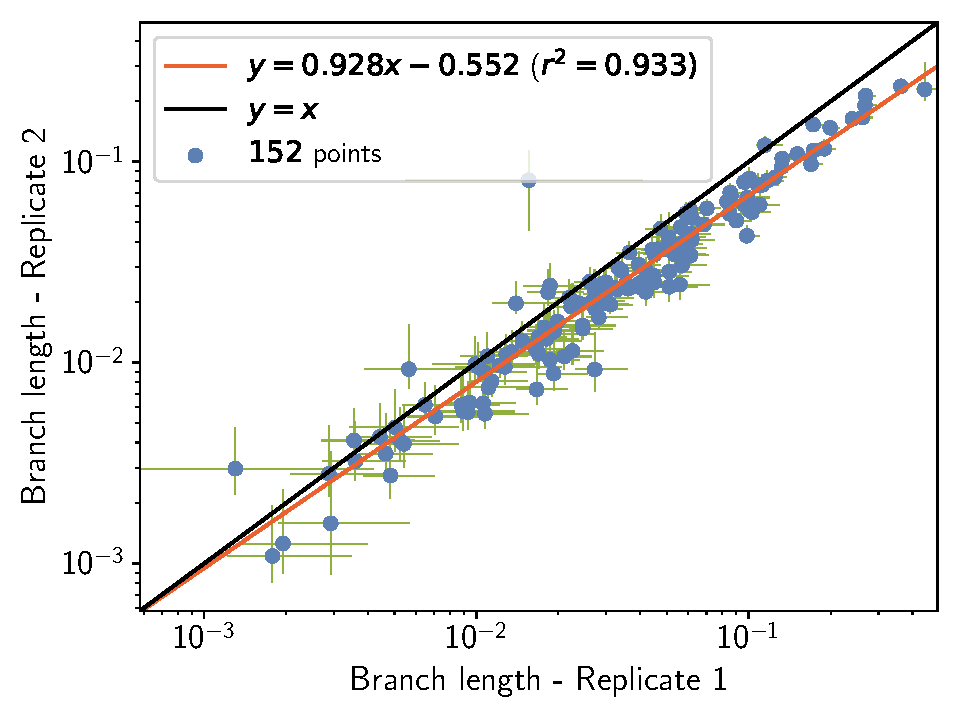
\includegraphics[width=\linewidth, page=1]{mammals/18CDS_SiteMutSelBranchNe_Rep_Log10BranchLength-1-2}
	\end{minipage}	\hfill
	\begin{minipage}{0.32\linewidth}
		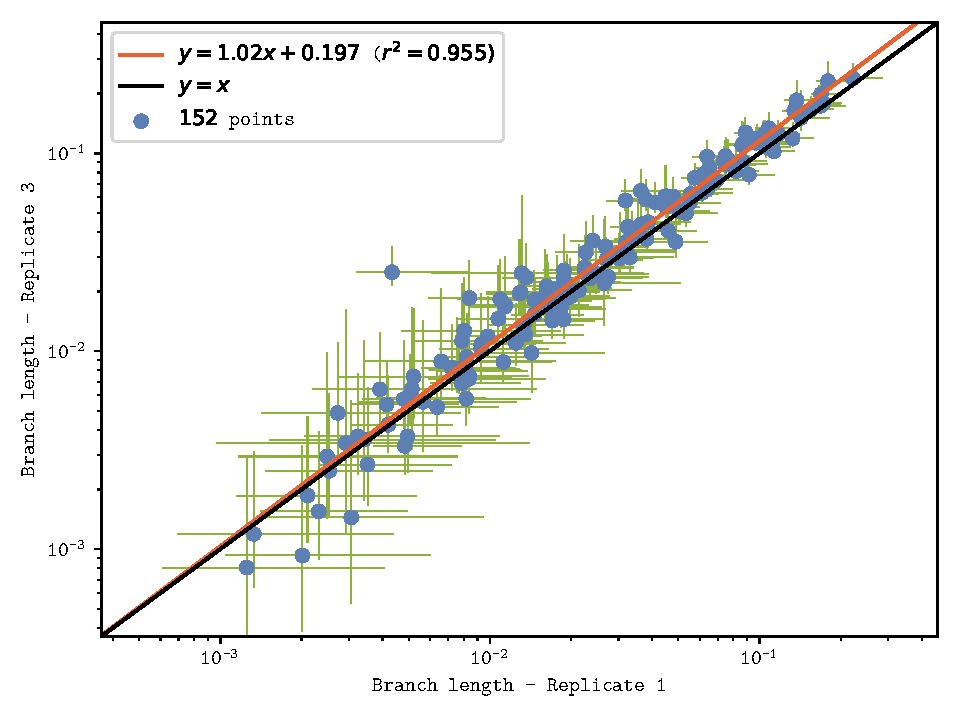
\includegraphics[width=\linewidth, page=1]{mammals/18CDS_SiteMutSelBranchNe_Rep_Log10BranchLength-1-3}
	\end{minipage}	\hfill
	\begin{minipage}{0.32\linewidth}
		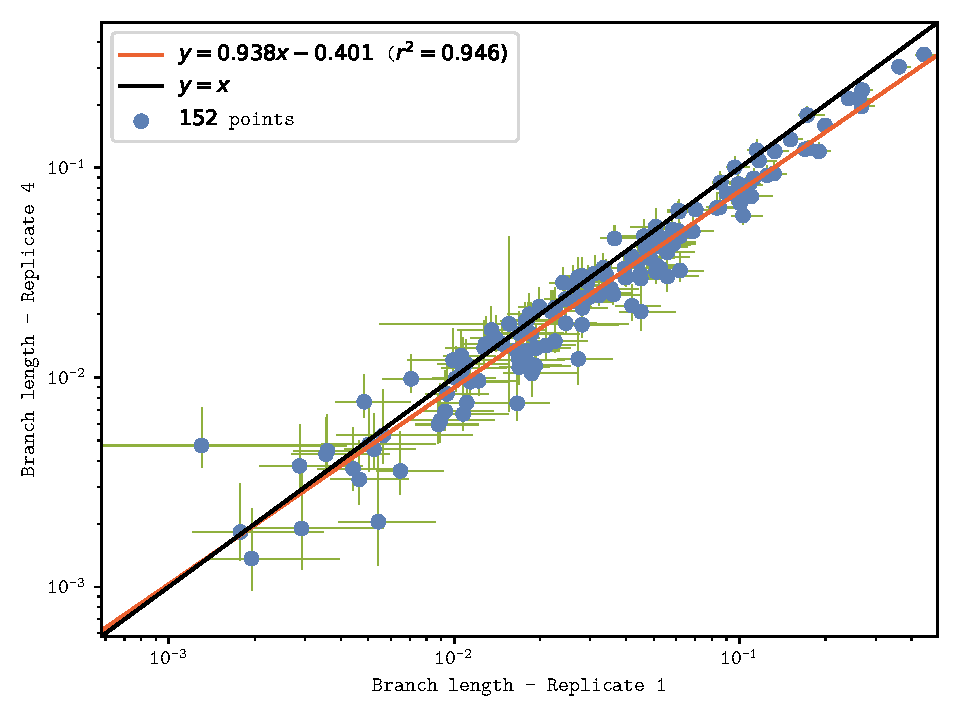
\includegraphics[width=\linewidth, page=1]{mammals/18CDS_SiteMutSelBranchNe_Rep_Log10BranchLength-1-4}
	\end{minipage}
	\begin{minipage}{0.32\linewidth}
		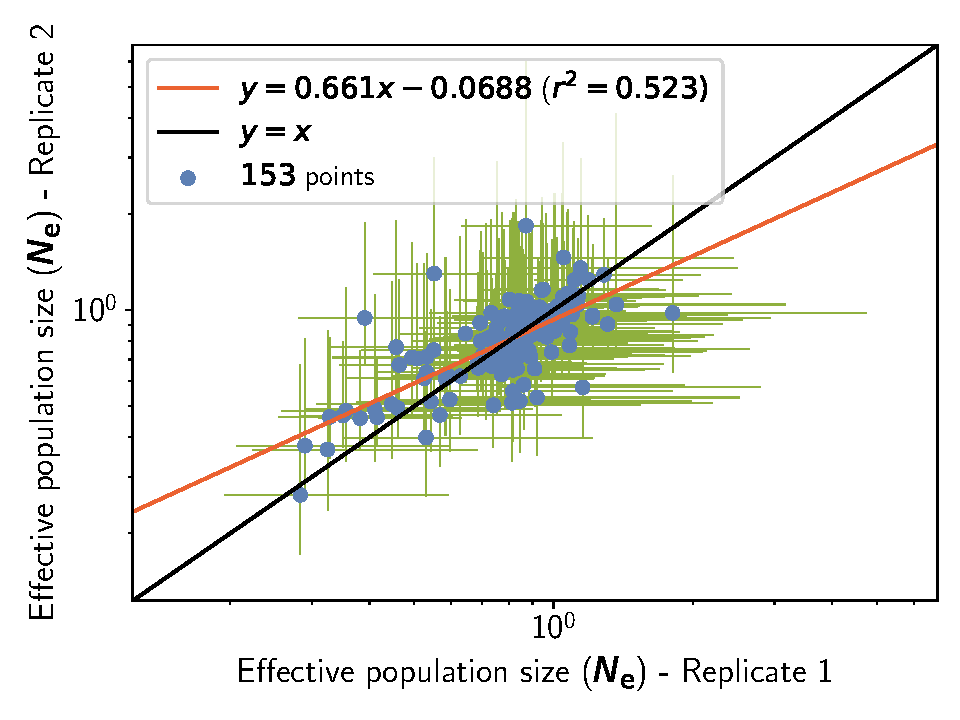
\includegraphics[width=\linewidth, page=1]{mammals/18CDS_SiteMutSelBranchNe_Rep_LogPopulationSize-1-2}
	\end{minipage}	\hfill
	\begin{minipage}{0.32\linewidth}
		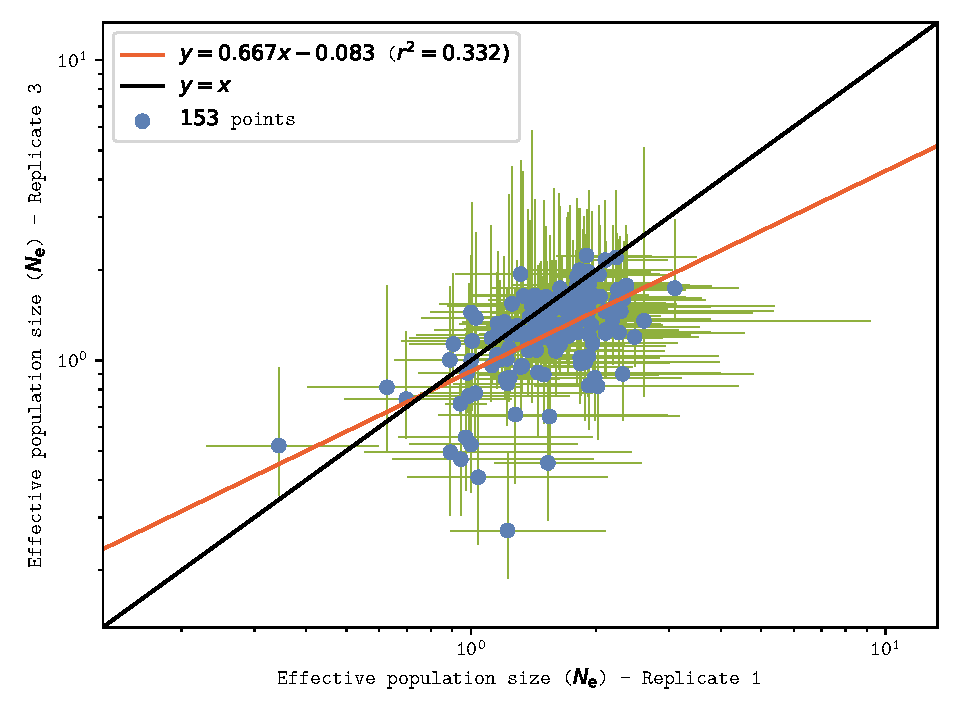
\includegraphics[width=\linewidth, page=1]{mammals/18CDS_SiteMutSelBranchNe_Rep_LogPopulationSize-1-3}
	\end{minipage}	\hfill
	\begin{minipage}{0.32\linewidth}
		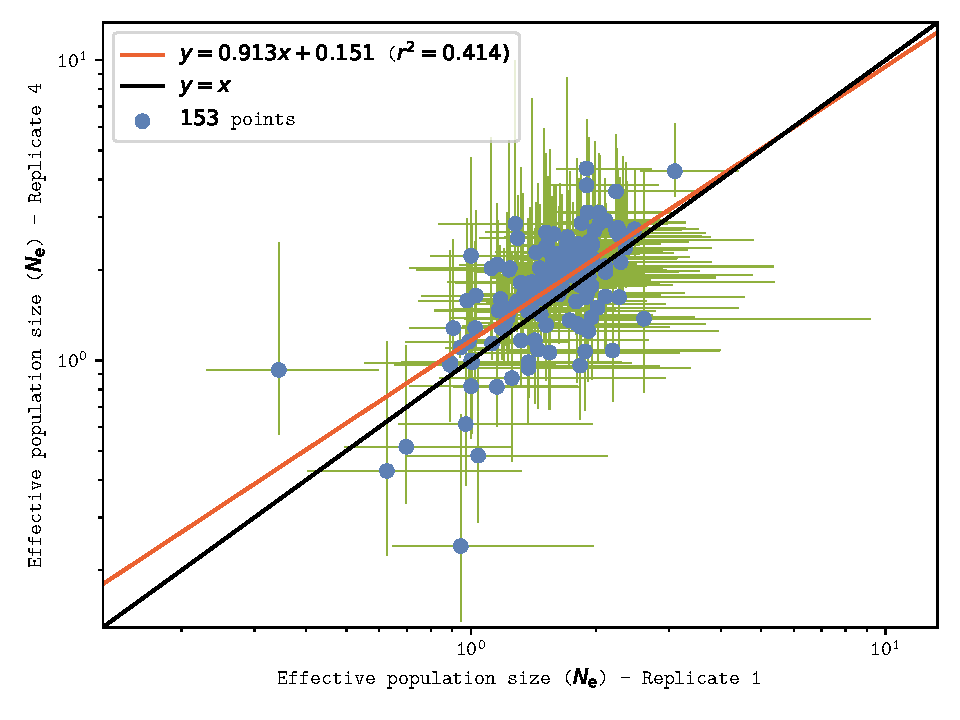
\includegraphics[width=\linewidth, page=1]{mammals/18CDS_SiteMutSelBranchNe_Rep_LogPopulationSize-1-4}
	\end{minipage}
	\caption[Repeatability of experiments]{
		Repeatability of experiments.
		$3$ independent inferences where performed on a randomly chosen set of $36$ coding sequences (CDS) out of $226$.
		Each plot is a correlation between a pair of experiments for a given parameter.
		$2$ relevant parameters are shown, mutation rate per unit of time~($\mu$, bottom left plots) and effective population size~($\Ne$, upper right plots).
		For each node of the tree, the mean of the parameter~($\Ne$ or $\mu$) over the \acrshort{MCMC} is represented in blue dot, green solid lines are the $90\%$ confidence interval of the \acrshort{MCMC}.
		Solid red line is the regression line between experiments.
		Inference of $\mu$ is more reproducible than $\Ne$, but overall the experiment is reproducible for a random subset of CDS.
	}
	\label{fig:mammals_repeatability}
\end{figure}

\section{Materials and Methods model}
\label{sec:MatMet}

\subsection{Nucleotide mutation rates}
The generalized time-reversible nucleotide mutation rate matrix $\Mutmatrix$ is a function of the nucleotide frequencies $\Mutequi$ and the relative rate $\Exchan$.
$\Mutequi = (\mutequi_A , \mutequi_C , \mutequi_G , \mutequi_T)$ is the equilibrium base frequency vector, giving the frequency at which each base occurs at each site.
$\Exchan = \left( \exchan_{AC}, \exchan_{AG}, \exchan_{AT}, \exchan_{CG}, \exchan_{CT}, \exchan_{GT}\right)$ is the vector of exchangeabilities between nucleotides.
Altogether, the rate matrix is:
\begin{equation}
\label{eq:gtr-mutrates}
\Mutmatrix =
	\begin{pmatrix}
		 - & {\exchan_{AC}\mutequi_C} & {\exchan_{AG}\mutequi_G} & {\exchan_{AT}\mutequi_T} \\
			 {\exchan_{AC}\mutequi_A} &                        - & {\exchan_{CG}\mutequi_G} & {\exchan_{CT}\mutequi_T} \\
			 {\exchan_{AG}\mutequi_A} & {\exchan_{CG}\mutequi_C} &                        - & {\exchan_{GT}\mutequi_T} \\
			 {\exchan_{AT}\mutequi_A} & {\exchan_{CT}\mutequi_C} & {\exchan_{GT}\mutequi_G} & -
	\end{pmatrix}
\end{equation}
By definition, the sum of the entries in each rows of the nucleotide rate matrix $\Mutmatrix$ is equal to $0$, giving the diagonal entries:
\begin{equation}
\mutmatrix_{a,a} = - \sum\limits_{ b \neq a} \mutmatrix_{a,b}
\end{equation}
The \gls{prior} on the exchangeabilities $\Exchan$ is a uniform Dirichlet distribution of dimension $6$:
\begin{equation}
\label{eq:DistribExchan}
\Exchan \sim \mathrm{Dir}\left( \dfrac{1}{6} , 6\right).
\end{equation}
The \gls{prior} on the equilibrium base frequencies $\Mutequi$ is a uniform Dirichlet distribution of dimension $4$:
\begin{equation}
\label{eq:DistribMutequi}
\Mutequi \sim \mathrm{Dir}\left( \dfrac{1}{4} , 4\right)
\end{equation}
The general time-reversible nucleotide matrix is normalized such that the total flow equals to $1$:
\begin{equation}
\sum\limits_{a \in \{A, C, G, T\}} - \mutequi_a \mutmatrix_{a,a} = 1.
\end{equation}

\subsection{Site-dependent selection}
\label{sec:profiles}
For each category $\Setcat$, a $20$-dimensional fitness profile $\Base\catexp$ (summing to $1$) is distributed as a Dirichlet of center $\Basecenter$ and concentration $\baseconc$:
\begin{equation}
\label{eq:DistribBase}
\Base\catexp \sim \mathrm{Dir}\left( \Basecenter,\ \baseconc \right),\ \Setcat.
\end{equation}
For an alignment of size $\Nsite$, each site $\Setsite$ is assigned a fitness profile category of amino-acids $\catsite \in \catInterval $.
The total number of sites falling in each fitness profile category $\cat$ is denoted $\catmultivar_{\cat}$.
The $\Ncat$-dimensional vector $\catMultiVar$ is distributed as a Multinomial of event probabilities $\StickBreaking$:
\begin{align}
\label{eq:DistribMultinomial}
\catMultiVar \sim \mathrm{Multinomial}\left( \StickBreaking \right).
\end{align}
The event probabilities $\Ncat$-dimensional vector~($\StickBreaking$) of falling into each category is distributed as a stick-breaking \gls{Dirichlet-process}:
\begin{align}
\label{eq:DistribStickBreaking}
\begin{split}
& \StickBreaking \sim \mathrm{StickBreaking}\left( \Ncat, \stickbreakinghyper \right)\\
\iff & \stickbreaking_{\cat} = \stick_{\cat}\cdot \prod _{{\indice=1}}^{{\cat-1}}\left(1-\stick_{\indice}\right),\ \Setcat,
\end{split}
\end{align}
where $\stick_{\cat}$ are i.i.d.
from a beta distribution
\begin{equation}
\label{eq:Beta}
\stick_{\cat} \sim \mathrm{Beta}\left( 1, \stickbreakinghyper \right),\ \Setcat.
\end{equation}
The Malthusian fitness selection coefficients $\Fit\siteexp$ at site $\site$, are obtained by taking the logarithm of the fitness profile assigned to this site:
\begin{equation}
\label{eq:sitefitness}
\Fit\siteexp = \log \left( \Base^{\left( \catsite \right)} \right),\ \Setsite.
\end{equation}

\subsection{Dated tree}
The topology of the rooted phylogenetic tree is supposed to be known and is not estimated by the model. The model estimates the dates at which branches split, thus the dated tree requires $\Ntaxa - 2$ internal node ages that are free parameters, where $\Ntaxa$ is the number of extant taxa (leaves of the tree). 
The node ages $\age\nodeexp,\ \Setinternal$ are drawn uniformly such that a node can not be younger than the oldest of its $2$ descendant children, and must also be younger than its parent:
\begin{equation}
\label{eq:Distribage}
\age\nodeexp \ \sim \mathcal{U}\left( \mathrm{max}\left(\age^{(\mathrm{children})} \right), \age^{(\mathrm{parent})} \right)
\end{equation}
By definition, leaf ages are all set to $0$. The root age is set arbitrarily to $1$, but if fossils data are also available the dated tree can be re-scaled into absolute time using cross-multiplication.\\
The duration of the branch~($\branchtime\branchexp$), for each branch $\Setbranch$ is defined as the difference in ages between the oldest node at the tip of the branch $\age^{(\nodeUp)}$, and the youngest node $\age^{(\nodeDown)}$:
\begin{equation}
\label{eq:ageTobranchtime}
\branchtime\branchexp = \age^{(\nodeUp)} - \age^{(\nodeDown)}.
\end{equation}
\subsection{Branch dependent traits}
The \gls{effective-population-size} $\Ne$ and mutation rate per unit of time $\mu$ are assumed to evolve along the phylogeny, and to be correlated.
If quantitative life-history-traits (LHT) are also available for some nodes of the tree (leaves and/or internal nodes), they are also assumed to evolve along the phylogeny and to be correlated between them, and with $\Ne$ and $\mu$.
The total number of traits (counting $\Ne$, $\mu$ and all user defined LHT) is denoted $\Ntrait$.
Their fluctuations are modelled by a $\Ntrait$-dimensional log-Brownian process $\Brownian\nodeexp$ at each node $\Setnode$ of the tree, including the root and leaves.
The first dimension (indiced by $0$) of the log-Brownian contain $\Ne$, and the second dimension (indiced by $1$) contains $\mu$.
The log-Brownian process and variables of interest~($\mu$ and $\Ne$) are linked by an exponential transformation:
\begin{equation}
\begin{dcases}
\Ne\nodeexp = \e^{ \brownian_{0}\nodeexp } \\ 
\mu\nodeexp = \e^{ \brownian_{1}\nodeexp },
\end{dcases}
\end{equation}
where the \gls{effective-population-size} at the root is set to $1$ for identifiability of the fitness profiles.
It is important to note that inferred correlation between $\Ne$, $\mu$ and other LHT is thus in the log space, and that quantitative LHT must be inputted in log scale.

Along a branch $\Setbranch$ of the tree, a log-Brownian process starts at the oldest node at the tip of the branch~($\nodeUp$), and ends at the youngest node~($\nodeDown$).
However we are interested in the average over the branch to define the \gls{codon} \gls{substitution} matrices along the branch.
In the case of log-Brownian process, the most likely path (or geodesic) from $\Brownian^{(\nodeUp)}$ to $\Brownian^{(\nodeDown)}$ is the straight line, and therefore, it would make sense to take the mean value of $\e^{\Brownian\nodeexp}$ along this geodesic.
We then have $\Ne\branchexp$ and $\mu\branchexp$ for each branch $\Setbranch$ of the tree:
\begin{equation}
\label{eq:branchNemu}
\begin{dcases}
\Ne\branchexp = \dfrac{\e^{\brownian_{0}^{(\nodeDown)}} - \e^{\brownian_{0}^{(\nodeUp)}}}{\brownian_{0}^{(\nodeDown)} - \brownian_{0}^{(\nodeUp)}} \\ 
\mu\branchexp = \dfrac{\e^{\brownian_{1}^{(\nodeDown)}} - \e^{\brownian_{1}^{(\nodeUp)}}}{\brownian_{1}^{(\nodeDown)} - \brownian_{1}^{(\nodeUp)}}.
\end{dcases}
\end{equation}

Moreover, the rate of change of the log-Brownian process per unit of time is constant and determined by the positive semi-definite and symmetric covariance matrix $\CovarianceMatrix$, and thus the distribution of $\Brownian^{(\nodeDown)}$ is multivariate Gaussian, with mean $\Brownian^{(\nodeUp)}$ and variance $\branchtime\branchexp \CovarianceMatrix$:
\begin{equation}
\label{eq:DistribBrownian}
\Brownian^{(\nodeDown)} \sim \mathcal{N}\left(\Brownian^{(\nodeUp)}, \branchtime\branchexp \CovarianceMatrix \right),\ \Setbranch
\end{equation}

\begin{figure}[H]
	\centering
		\begin{tikzpicture}[->,>=stealth',shorten >=1pt,auto,node distance=0.6cm and 1.2cm,semithick]
		\tikzstyle{every state}=[]
		
		\node[state] (P) {$\Probmatrix\branchsiteexp$};
		\node[state] (Q) [below right=of P] {$\Submatrix\branchsiteexp$};
		\node[state] (R) [below right=of Q] {$\Mutmatrix$};
		\node[state] (BL) [above right=of P] {$\branchlength\branchexp$};
		\node[state] (Ne) [above right=of Q] {$\Ne\branchexp$};
		\node[state] (Bb) [above right=of Ne] {$\Brownian\nodeexp $};
		\node[state] (Mu) [left=of Bb] {$\mu\branchexp$};
		\node[state] (f) [right=of Q] {$\Fit\siteexp $};
		\node[state] (Ex) [BLUE, below right=of R] {$\Exchan$};
		\node[state] (Equi) [BLUE, right=of R] {$\Mutequi$};
		\node[state] (dT) [above left=of Bb] {$\branchtime\branchexp $};
		\node[state] (T) [BLUE, right=of dT] {$\age\nodeexp$};
		\node[state] (Base) [BLUE, above right=of f] {$\Base\catexp$};
		\node[state] (cat) [BLUE, right=of f] {$\catsite$};
		\node[state] (ExH) [RED, right=of Ex] {$\dfrac{1}{6}, 6$};
		\node[state] (EquiH) [RED, right=of Equi] {$\dfrac{1}{4}, 4$};
		\node[state] (Unif) [RED, right=of T] {$\uniform$};
		\node[state] (C) [BLUE, right=of Bb] {$\contrast\branchexp$};
		\node[state] (Cov) [BLUE, right=of C] {$\Covariancematrix$};
		\node[state] (baseH) [RED, right=of Base] {$\baseconc, \Basecenter $};
		\node[state] (sb) [BLUE, right=of cat] {$\StickBreaking$};
		\node[state] (CovH) [RED, right=of Cov] {$\covariancekappa, \covariancedf$};
		\node[state] (sbH) [RED, right=of sb] {$\stickbreakinghyper$};
		
		\path 
		(Q) edge [dashed] node [above right] {\ref{eq:Probmatrix}} (P)
		(dT) edge [dashed] node [above left] {\ref{eq:branchlength}} (BL)
		(Mu) edge [dashed] node [] {} (BL)
		(BL) edge [dashed] node [] {} (P)
		(Ne) edge [dashed] node {} (Q)
		(R) edge [dashed] node {} (Q)
		(Bb) edge [dashed] node {} (Ne)
		(Bb) edge [dashed] node [below] {\ref{eq:branchNemu}} (Mu)
		(f) edge [dashed] node [above] {\ref{eq:subrates}} (Q)
		(Ex) edge [dashed] node [] {} (R)
		(Equi) edge [dashed] node [below] {\ref{eq:gtr-mutrates}} (R)
		(T) edge [dashed] node [above] {\ref{eq:ageTobranchtime}} (dT)
		(dT) edge [dashed] node {} (Bb)
		(Base) edge [dashed] node {} (f)
		(cat) edge [dashed] node [above] {\ref{eq:sitefitness}} (f)
		(ExH) edge [BLUE] node [above] {\ref{eq:DistribExchan}} (Ex)
		(EquiH) edge [BLUE] node [above] {\ref{eq:DistribMutequi}} (Equi)
		(Unif) edge [BLUE] node [above] {\ref{eq:Distribage}} (T)
		(C) edge [dashed] node [above] {\ref{eq:independent_contrast}} (Bb)
		(Cov) edge [BLUE] node [above] {\ref{eq:Distribcontrast}} (C)
		(baseH) edge [BLUE] node [above] {\ref{eq:DistribBase}} (Base)
		(sb) edge [BLUE] node [above] {\ref{eq:DistribMultinomial}} (cat)
		(CovH) edge [BLUE] node [above] {\ref{eq:Distribcovariance}} (Cov)
		(sbH) edge [BLUE] node [above] {\ref{eq:DistribStickBreaking},\ref{eq:Beta}} (sb);
		\end{tikzpicture}

	\caption[Directed acyclic graph of dependencies between variables]{
	Directed acyclic graph of dependencies between variables.
	Nodes of the directed acyclic graph are the variables, and edges are the functions.
	Hyper-parameters are depicted in {\color{RED}{red}} circle, random variables in {\color{BLUE}{blue}} circles, and transformed variables in black.
	Solid {\color{BLUE}{blue}} line denotes a drawing from a random distribution, and black dashed lines denote a function.
}
	\label{fig:graph}%
\end{figure}

We make a change of variable as to define the branch-wise independent contrast $\contrast\branchexp$:
\begin{align}
\contrast\branchexp &= \dfrac{\brownian^{(\nodeDown)} - \brownian^{(\nodeUp)}}{\sqrt{\branchtime\branchexp}} \\
\label{eq:independent_contrast}
\iff \brownian^{(\nodeDown)} &= \brownian^{(\nodeUp)} + \sqrt{\branchtime\branchexp}\contrast\branchexp 
\end{align}
And these contrasts are i.i.d.
from a multivariate normal distribution:
\begin{equation}
\label{eq:Distribcontrast}
\contrast\branchexp \sim \mathcal{N}\left(\bm{0}, \Covariancematrix \right), \Setbranch
\end{equation}
The \gls{prior} on the covariance matrix is an invert Wishart distribution, parameterized by $\covariancekappa=1$ and with $\covariancedf=\Ntrait + 1$ degrees of freedom:
\begin{equation}
\label{eq:Distribcovariance}
\CovarianceMatrix \sim \mathrm{Wishart}^{-1} (\covariancekappa \Identitymatrix, \covariancedf)
\end{equation}

\subsection{Codon {substitution} rates}
For a given branch $\branch$ and a given site $\site$, the \gls{codon} \gls{substitution} rate (per unit of time) matrix $\Submatrix\branchsiteexp$ is given by:
\begin{equation}
\label{eq:subrates}
\begin{dcases}
\submatrix\branchsiteexp_{\itoj} = 0\text{ if $\ci$ and $\cj$ are not neighbors,} \\
\submatrix\branchsiteexp_{\itoj} = \mutmatrix_{\nucitoj}\text{ if $\ci$ and $\cj$ are synonymous,} \\
\submatrix\branchsiteexp_{\itoj} = \mutmatrix_{\nucitoj} \dfrac{4\Ne\branchexp \left({\fitj\siteexp - \fiti\siteexp}\right)}{{1 - \e^{4\Ne\branchexp\left({\fiti\siteexp - \fitj\siteexp}\right)} }} \text{ if non-syn.,}\\
\submatrix\branchsiteexp_{\ci, \ci} = - \sum\limits_{ \cj \neq \ci, \jSetCodon} \submatrix\branchsiteexp_{\itoj},
\end{dcases}
\end{equation}
The branch length $\branchlength\branchexp$ are defined as the expected number of \gls{neutral} \glspl{substitution} per \acrshort{DNA} site along a branch:
\begin{equation}
\label{eq:branchlength}
\branchlength\branchexp = \mu\branchexp \branchtime\branchexp
\end{equation}
Together, the probability of {transition} between \glspl{codon} for a given branch $\branch$ and site $\site$ is:
\begin{equation}
\label{eq:Probmatrix}
\Probmatrix\branchsiteexp = \e^{\branchlength\branchexp \Submatrix\branchsiteexp},
\end{equation}
which are the matrices necessary to compute the \gls{likelihood} of the data $\data$ given the parameters of the model using the pruning algorithm (Supplementary Materials).

\subsection{Bayesian implementation}
\label{sec:Bayesian}
The \gls{likelihood} computed by the pruning algorithm can then be combined with the \gls{prior} over the model parameters.
A realization of the random process results in a detailed \gls{substitution} history over the tree.
Most phylogenetic Monte-Carlo-Markov-Chain (\acrshort{MCMC}) samplers target the distribution over the model parameters, which means that they have to repeatedly invoke the pruning algorithm to recalculate
the pruning-based \gls{likelihood} which is most often the limiting step of the \acrshort{MCMC}.

An alternative, which is used here, is to do the \acrshort{MCMC} conditionally on the detailed \gls{substitution} history $\subhistory$, thus doing the \acrshort{MCMC} over the augmented configuration~($\subhistory$, $\data$), under the target distribution obtained by combining the mapping-based \gls{likelihood} with the \gls{prior} over model parameters

The key idea that makes this strategy efficient is that the mapping-based \gls{likelihood} depends on
compact summary statistics of $\subhistory$ (which in turn depend on the specific parameter component
being resampled), leading to very fast evaluation of the \gls{likelihood}.
On the other hand, this requires to implement more complex \acrshort{MCMC} procedures, that have to alternate between:

1) sampling $\subhistory$ conditionally on the data and the current parameter configuration.

2) re-sampling the parameters conditionally on $\subhistory$.

To implement the mapping-based \acrshort{MCMC} sampling strategy, we first sample the detailed \gls{substitution} history $\subhistory$ for all sites along the tree.
Several methods exist for doing this~\citep{Nielsen2002,Rodrigue2008}.
Then, we write down the probability of $\subhistory$ given the parameters, and finally, we collect all factors that depend on some parameter of interest and make some simplifications.
This ultimately leads to relatively compact sufficient statistics (Supplementary Materials for the different sufficient statistics used by our model) that are fast to evaluate~\citep{Irvahn2014,Davydov2016}.

As an example, making an \acrshort{MCMC} move on the $\Ne$ at a given node of the tree is drastically faster since only the mapping-based \gls{likelihood} (using path sufficient statistics) at the neighboring branches of the node is necessary, and not computing the \gls{likelihood} for the all tree.
\\

\subsection{Correlation between traits}
\label{sec:Correlation}
The correlation between traits $\Settrait$ and trait $\traitj \in \traitInterval$ can be obtained from the covariance matrix $\Covariancematrix$:
\begin{equation}
\rho_{\traiti, \traitj} = \dfrac{\Covariancematrix_{\traiti, \traitj}}{\sqrt{\Covariancematrix_{\traiti, \traiti} \Covariancematrix_{\traitj, \traitj}}}
\end{equation}

\subsection{Simulations}
\label{sec:Simulation}
To test the robustness of the model, $3$ parameterized simulators were developed: \textit{SimuDiv}, \textit{SimuPoly} \& \textit{SimuFold}.
All $3$ simulators use a log-Brownian multivariate process to model conjointly the changes in mutation rate per generation, the generation time and $\Ne$, in logarithm space.
\textit{SimuDiv} \& \textit{SimuFold} both simulate point \glspl{substitution} along the phylogenetic tree.
The simulator starts from an initial sequence at equilibrium.
The change in fitness is computed for all possible mutant, hence computing all strictly positive \gls{substitution} rates.
At each point, the next \gls{substitution} is chosen proportional to the rate as in Gillespie algorithm.
At each node, the process is split, and finally the process is stopped at the leaves of the tree.
\textit{SimuPoly} simulates explicitly each generation along the phylogeny under a Wright-Fisher population, consisting of three steps: mutation, selection and random drift of \glspl{allele}.
Mutations are drawn randomly based on the probability of mutation.
Drift is modeled as a multinomial distribution on the \gls{allele} counts.
We assumed that the \acrshort{DNA} sequence is composed of exons, with no linkage between exons, and total linkage of sites within an exon.
Moreover, in \textit{SimuPoly} $\Ne$ can also be modeled as a sum of a log-Brownian process and an Ornstein-Uhlenbeck process.
The log-Brownian motion takes into account long-term fluctuations, while the Ornstein-Uhlenbeck can take into account short fluctuations of $\Ne$.
In \textit{SimuDiv} and \textit{SimuPoly} each \gls{codon} site contribute independently to the fitness depending on the encoded amino-acids, through site-specific amino-acid fitness profiles experimentally determined~\citep{Bloom2017}.
However, in \textit{SimuFold} the fitness of a sequence is computed as the probability of the protein to be in the folded state (Supplementary Materials).
\textit{SimuFold} is in practice a C++ adaptation of a Java code previously published~\citep{Goldstein2016, Goldstein2017}, where we allow for changes in $\Ne$ and $\mu$ along a phylogenetic tree.

The simulators written in C++ are publicly available under MIT license at \url{https://github.com/ThibaultLatrille/SimuEvol}
